\documentclass{report}

% Packages
\usepackage{import}
\usepackage{xcolor}
\usepackage{cancel}
\usepackage{mathtools}
\usepackage{hyperref}
\usepackage{setspace}
\usepackage{float}
\usepackage{parskip}
\setlength{\parindent}{0pt}

% Custom perms and combs commands
\newcommand\Myperm[2][^n]{\prescript{#1\mkern-2.5mu}{}P_{#2}}
\newcommand\Mycomb[2]{\prescript{#1\mkern-0.5mu}{}C_{#2}}

% Colors
\definecolor{yorhabg}{HTML}{131314}
\definecolor{yorhafg}{HTML}{C9C7CD}
\definecolor{yorhagrid}{HTML}{B5AF9C}
\definecolor{mred}{HTML}{D67069}
\definecolor{mblue}{HTML}{6887A1}

\usepackage[dvipsnames]{xcolor}
\definecolor{pastel_red}{RGB}{255, 173, 173}
\definecolor{pastel_orange}{RGB}{255, 214, 165}
\definecolor{pastel_yellow}{RGB}{253, 255, 182}
\definecolor{pastel_green}{RGB}{176, 217, 176}
\definecolor{pastel_blue}{RGB}{167, 199, 231}
\definecolor{pastel_purple}{RGB}{222, 218, 244}

\pagecolor{yorhabg}		% Set background color
\color{yorhafg}

\import{preamble.sty}

\usepackage[T1]{fontenc}			% Font package

\usepackage{fouriernc}

\usepackage{sectsty}
\usepackage{graphicx}
\usepackage{amsmath}
\usepackage{amsfonts}
\usepackage{amssymb}
\usepackage[skins, most]{tcolorbox}

\DeclareMathOperator{\sgn}{sgn}

\DeclareMathOperator{\area}{area}
\DeclareMathOperator{\sech}{sech}
\DeclareMathOperator{\cosech}{cosech}
\usepackage{tikz}
\usepackage{eso-pic}
\usetikzlibrary{calc, shadows.blur}
\usetikzlibrary{angles, quotes}
\usetikzlibrary{3d}

% Margins
\topmargin=0in
\evensidemargin=0in
\oddsidemargin=0in
\textwidth=6.5in
\textheight=9.0in
\headsep=0.25in

\AtBeginEnvironment{tcolorbox}{\small}

\newtcolorbox{imp}{enhanced,arc=0mm,colback=yorhabg,colframe=mred,leftrule=10mm,coltext=yorhafg,%
overlay={\node[anchor=west,outer sep=2pt] at (frame.west) {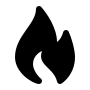
\includegraphics[width=6mm]{images/imageb.png}}; }}

\newtcolorbox{shortcut}{enhanced,arc=0mm,colback=yorhabg,colframe=mred,leftrule=10mm,coltext=yorhafg, coltitle=yorhabg, title=\texttt{Shortcut.}, 
overlay={\node[anchor=west,outer sep=2pt] at (frame.west) {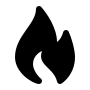
\includegraphics[width=6mm]{images/imageb.png}}; }}

\newtcolorbox{question}[1]{
    enhanced, 
    colback=yorhabg,
    colframe=mblue,
    coltext=yorhafg,
    coltitle=yorhabg,
    attach boxed title to top left={yshift*=-\tcboxedtitleheight}, 
    title=\texttt{#1},
    boxed title size=title,
    boxed title style={%
        rounded corners=northeast, 
        rounded corners=northwest, 
        colback=tcbcolframe, 
        boxrule=0pt,
    },
    underlay boxed title={%
        \path[fill=tcbcolframe] (title.south west)--(title.south east) 
            to[out=0, in=180] ([xshift=5mm]title.east)--
            (title.center-|frame.east)
            [rounded corners=5pt] |- 
            (frame.north) -| cycle; 
    },
}

\newcommand\bb[1]{\textcolor{yorhafg}{\textbf{#1}}}

\title{\textbf{MATH1141: Higher Mathematics 1A (Calculus)}}
\author{L. Cheung}
\date{\today}

\begin{document}

\maketitle
\tableofcontents
\newpage

\chapter{Sets, inequalities and functions}
	\section{Sets of numbers}
		A \textcolor{pastel_blue}{set} is a collection of distinct objects. The objects in a set are elements or members of the set. Commonly used sets:
			\begin{itemize}
				\item The set of natural numbers: $\mathbb{N} = \{0, 1, 2, 3, 4,...\}$
				\item The set of integers: $\mathbb{Z} = \bigl\{...,-3,-2,-1,0,1,2,3,...\}$
				\item The set of rational numbers: $\mathbb{Q} = \{\frac{p}{q}: p,q \text{ are integers and } q \neq 0\}$
				\item The set of $\mathbb{R}$ real numbers may be represented as the collection of points lying on the number line
			\end{itemize}
		If $A$ is a set of numbers and the number $x$ is a member of the set $A$, then we write:
			\begin{align*}
				x \in A
			\end{align*}

		If $x$ is not a member of $A$, then we write
			\begin{align*}
				x \notin A
			\end{align*}


	\subsection{Intervals}
		\begin{itemize}
			\item Parenthesis: excludes endpoints
			\item Bracket: includes endpoints
			\item Combination: neither open nor closed interval
		\end{itemize}

	\subsection{Solving Inequalities}
		For $x, y, z \in \mathbb{R}$:
			\begin{itemize}
				\item if $x>y$, then $x+z>y+z$ 
				\item if $x>y$ and $z>0$, then $xz>yz$
				\item if $x>y$ and $z<0$, then $xz<yz$
			\end{itemize}

		\begin{question}{Example}
			Solve the quadratic inequality $x^2 + 4x > 21$
			\begin{align*}
				x^2 + 4x > 21 & \Longleftrightarrow x^2+4x-21>0 \\
							  & \Longleftrightarrow (x+7)(x-3)>0 \\
				\text{Solution set: } & x < -7 \text{ or } x > 3 \\
									  & x \in (-\infty, -7) \cup (3, \infty)			\end{align*}
		\end{question}

		\begin{question}{Example}
			Solve the rational inequality $\frac{1}{x+1}<\frac{1}{(x-2)(x-2)}$
			\begin{align*}
				\text{Multiply both sides by } & (x+1)^2(x-2)^2(x-3)^2 \quad  (>=0), \\
				\frac{1}{x+1}<\frac{1}{(x-2)(x-3)} & \Longleftrightarrow (x+1)(x-2)^2(x-3)^2 < (x+1)^2(x-2)(x-3) \\
												   & \Longleftrightarrow (x+1)(x-2)^2(x-3)^2 - (x+1)^2(x-2)(x-3) <0 \\
												   & \Longleftrightarrow (x+1)(x-2)(x-3)(x-4)(x-5) < 0 \\
							 \text{Solution set: } & (-\infty, -1) \cup (1,2) \cup (3,5)
			\end{align*}
		\end{question}

		\begin{figure}[H]
			\centering
			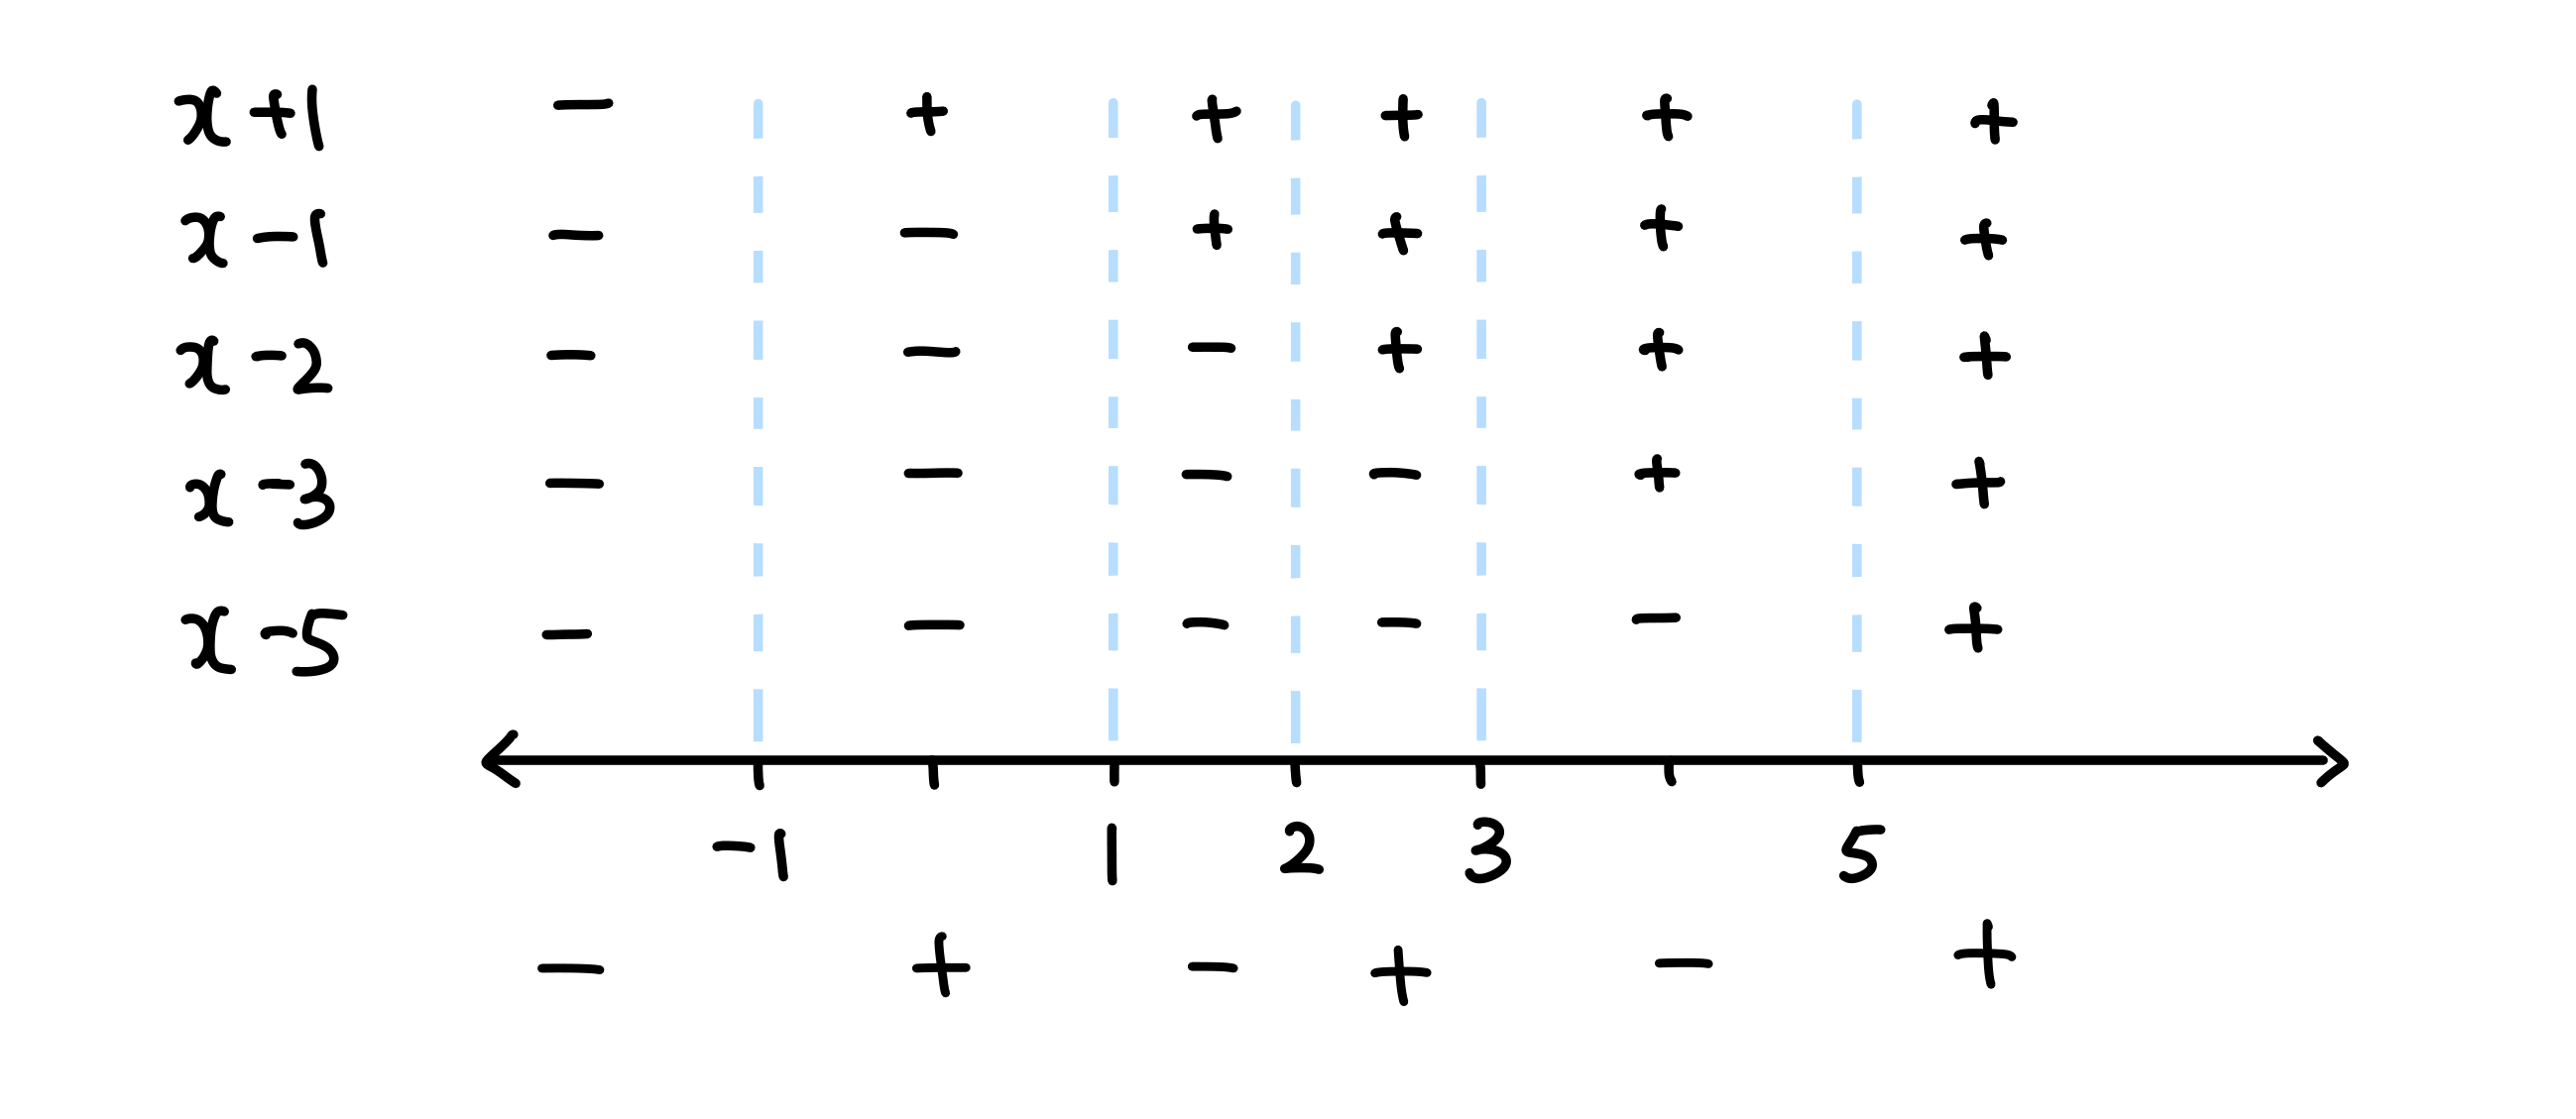
\includegraphics[width=0.6\textwidth]{images/fig1}
		\end{figure}

	\subsection{Absolute Values}
		The absolute value (or magnitude) of a real number $x$ is
			\begin{align*}
				|x| = \left\{
					\begin{aligned}
						x & \quad \text{if } x\leq0, \\
						-x& \quad \text{if } x<0
					\end{aligned}
			\end{align*}

		\begin{question}{Example}
			Solve the inequality $|3x+1| \leq 4$
			\begin{align*}
				|3x+1| \leq 4 & \Longleftrightarrow |x+ \frac{1}{3}| \leq \frac{4}{3} \\
							  & \Longleftrightarrow x + \frac{1}{3} \leq \frac{-4}{3} \quad \text{or} \quad x + \frac{1}{3} \leq \frac{4}{3} \\
							  & \Longleftrightarrow x \leq \frac{-5}{3} \quad \text{or} \quad x \leq 1 \\
				\text{Solution set: } (-\infty, \frac{-5}{3}] \cup [1, \infty)
			\end{align*}
		\end{question}

		\begin{question}{Example}
			Solve the inequality $\frac{|x+5|}{|x-11|} < 1$
			\begin{align*}
				\frac{|x+5|}{|x-11|}<1 & \Longleftrightarrow |x+5| < |x-11| \quad\text{(multiply both sides by |x-11|)} \\
									   & \Longleftrightarrow |x+5|^2 < |x-11|^2 \\
									   & \Longleftrightarrow x^2 + 10x + 25 < x^2 -22x + 121 \\
									   & \Longleftrightarrow 32x < 96 \\
									   & \Longleftrightarrow x < 3 \\
				\text{Solution set: } (-\infty, 3) \\
				\text{\textcolor{pastel_red}{Note:} 11 is not in the solution set}
			\end{align*}
		\end{question}

	\subsection{Functions}
		\subsubsection{Domain, codomain and range}
			Let $A$ and $B$ be subsets of $\mathbb{R}$: A function with domain $A$ and codomain $B$ is a rule which assigns to every $x \in A$ exactly one number $f(x) \in B$
			\begin{align*}
				& f: A \rightarrow B \\ 
				& f: A \ni x \mapsto f(x) \in B
			\end{align*}

			\begin{itemize}
				\item $A = \text{Dom}(f)$: set of all inputs
				\item $B = \text{Codom}(f)$: set that contains all the outputs
				\item Range of $f$: set of actual outputs, defined by:
					\begin{align*}
						\text{Range}(f) = \bigl\{f(x) \in B: x \in A \bigr\}
					\end{align*}
				\item Hence, $\text{Range}(f) \subseteq \text{Codom}(f)
				\item The \textcolor{pastel_red}{codomain does not have to be unique}
				\item The codomain is useful when the range is unknown
			\end{itemize}

			\begin{question}{Example}
				Given: $f: [0,\infty) \rightarrow \mathbb{R}, f(x) = 2+\sqrt{x}, \forall x \in [0,\infty)$ \\
				Then, $\text{Dom}(f) = [0,\infty), \text{ Codom}(f) = \mathbb{R}, \text{ and Range}(f) = [2,\infty)$
			\end{question}

			Natural domain (or maximal domain) of $f$ is the largest possible domain for which the rule makes sense (for real numbers)

	\subsubsection{Forming new functions}
		Let $A$, $B$, $C$ and $D$ be subsets of $\mathbb{R}$. Given two functions $f: A \rightarrow B$ and $g: A \rightarrow B$, then the functions
			\begin{align*}
				f+g,\quad f-g, \quad fg,\quad \displaystyle\frac{f}{g}
			\end{align*}

		are defined by the rules
			\begin{align*}
				(f+g)(x) &= f(x)+g(x),\quad \forall x \in A \\
				(f-g)(x) &= f(x)-g(x), \quad \forall x \in A \\
				(fg)(x) &= f(x)g(x), \quad \forall x \in A \\
				\Bigl(\frac{f}{g}\Bigr)(x) &= \frac{f(x)}{g(x)}, \quad \forall x \in \text{A provided that } g(x) ̸= 0.
			\end{align*}

		To form these new functions, the domains of both $f$ and $g$ must be the same

		Suppose that $f:C \rightarrow D$ and $g:A \rightarrow B$ are functions such that
			\begin{align*}
				\text{Range}(g) \subseteq \text{Dom}(f) = C
			\end{align*}

		Then the composition function $(f \circ g)(x) = f(g(x)),\quad \forall x \in A$

	\subsection{The Elementary Functions}
		Elementary functions are those that can be constructed by combining a finite number of polynomials, exponentials, logarithms, roots, trigonometric and inverse trigonometric functions via function composition ($\circ$), $+$, $-$, $\times$, and $\div$.

	\subsection{Implicitly Defined Functions}
		Many curves on the plane can be described by the points $(x,y)$ that satisfy some equation involving x and y. However, not all these curves are necessarily functions. Some cannot be expressed with a single $y$ term ($y = \dots$). In this case, the curve may be decomposed into two or more functions that are \textcolor{pastel_blue}{implicitly} defined by the curve.

	\subsection{Continuous Functions}
		In the below example, the $\tan{x}$ graph breaks at $x = -\frac{\pi}{2}, \frac{\pi}{2}, \dots$.

		\begin{figure}[H]
			\begin{center}
				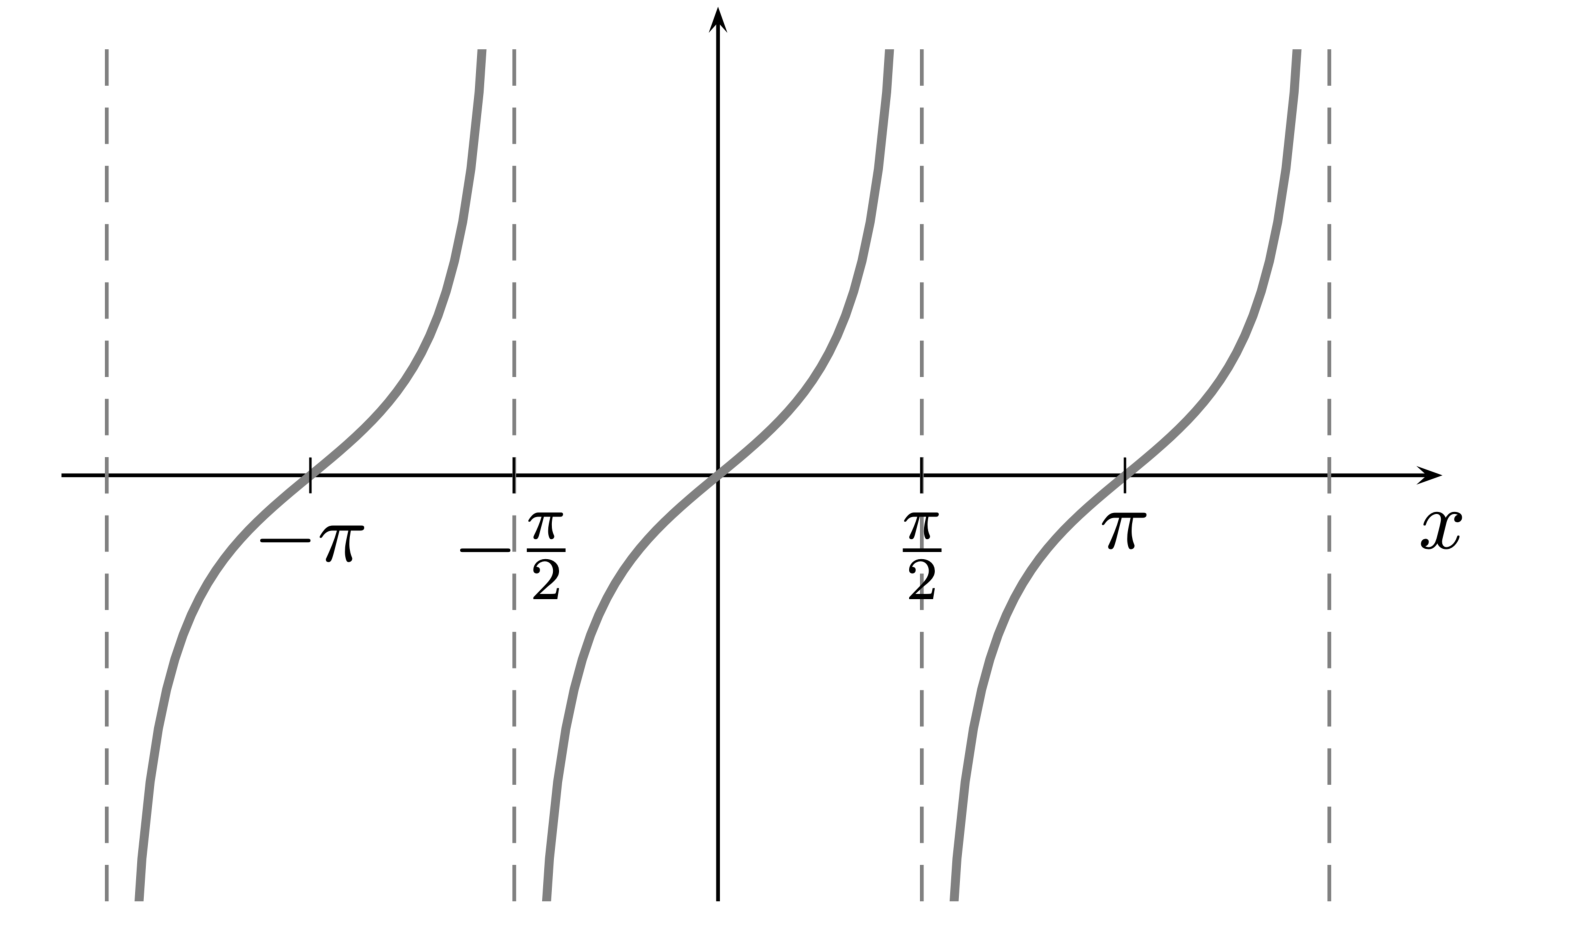
\includegraphics[width=0.7\textwidth]{images/tangraph.png}
			\end{center}
		\end{figure}

		However, this \textcolor{pastel_red}{break in the domain does not make it a discontinuity in the graph}. Discontinuities can be categorised as following:

		\begin{figure}[H]
			\begin{center}
				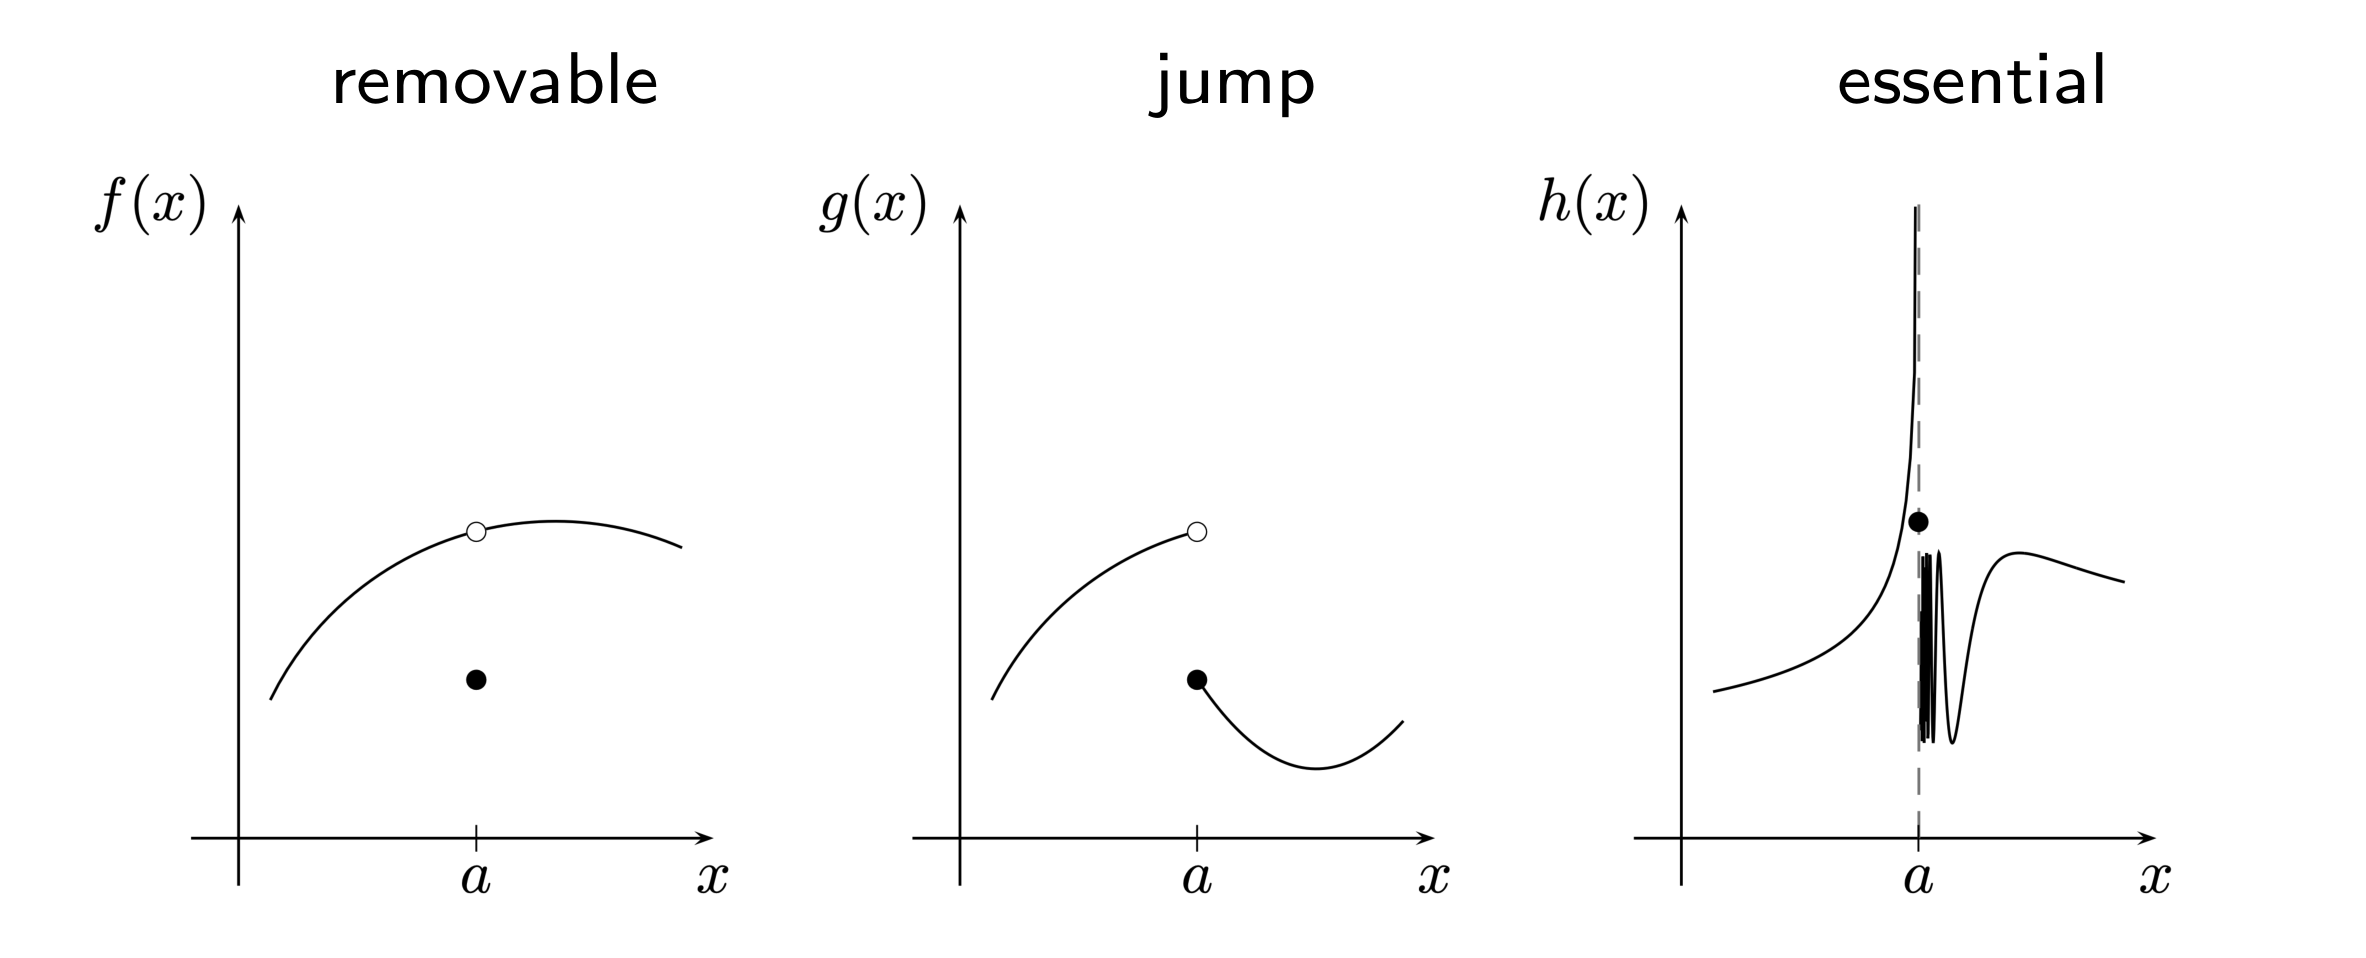
\includegraphics[width=0.95\textwidth]{images/discontinuities.png}
			\end{center}
		\end{figure}

\chapter{Limits}

\section{Limits of functions at infinity}

	\begin{itemize}
		\item If $f(x)$ gets arbitrarily close to some $L \in \mathbb{R}$ as $x$ tends to $\infty$, then we write:
			\begin{align*}
				\lim_{x\to\infty} f(x) = L \quad \text{or} \quad f(x) \rightarrow L \text{ as } x \rightarrow L
			\end{align*}
		\item If $f(x)$ gets arbitrarily large as $x$ tends to $\infty$, then we write:
			\begin{align*}
				f(x) \rightarrow \infty \text{ as } x \rightarrow \infty
			\end{align*}
			\begin{itemize}
				\item In this case, we state that the limit of $f(x)$ as $x$ tends to $\infty$ does not exist
					\begin{align*}
						\lim_{x\to\infty} \frac{1}{f(x)} = 0
					\end{align*}
			\end{itemize}
		\item The limit notation can only be used when the limit has a constant definition (do not write $\displaystyle\lim_{x\to\infty} = \infty$)
	\end{itemize}

	\subsection{Basic rules for limits}

		If $\displaystyle\lim_{x\to\infty} f(x) = L_1$ and $\displaystyle\lim_{x\to\infty} g(x) = L_2$ then 
		
		\begin{itemize}
			\item $\displaystyle\lim_{x\to\infty} (f(x) + g(x)) = L_1 + L_2$
			\item $\displaystyle\lim_{x\to\infty} (f(x) - g(x)) = L_1 - L_2$
			\item $\displaystyle\lim_{x\to\infty} f(x)g(x) = L_1L_2$
			\item $\displaystyle\lim_{x\to\infty} \frac{f(x)}{g(x)} = \frac{L_1}{L_2}$, provided that $L_2 \neq 0$
		\end{itemize}

		\begin{question}{Example}
			Find the limit of $f(x) = \frac{1 + \frac{2}{3x+4}}{5-6e^{-x}}$ as $x \rightarrow \infty$ (if it exists)

			\begin{align*}
				\lim_{x\to\infty} f(x) &= \frac{\displaystyle\lim_{x\to\infty}(1 + \frac{2}{3x+4})}{\displaystyle\lim_{x\to\infty}(5-6e^{-x})} \\
									   &= \frac{\displaystyle\lim_{x\to\infty}1 + \displaystyle\lim_{x\to\infty} \frac{2}{3x+4}}{\displaystyle\lim_{x\to\infty}5 - \displaystyle\lim_{x\to\infty}6e^{-x}} \\
									   &= \frac{1+0}{5-0} \\
									   &= \frac{1}{5}
			\end{align*}
		\end{question}

	\subsection{The pinching theorem}

		Suppose that $f$ and $h$ have the same limit as $x \rightarrow \infty$. If the graph of $g$ always lies between the graphs of $f$ and $h$, then $g$ has the same limit.

		\textbf{Theorem} Let $f$, $g$, and $h$ be functions defined on $(b,\infty)$ for some $b \in \mathbb{R}. If:$
		\begin{itemize}
			\item $f(x) \leq g(x) \leq h(x), \quad \forall x \in (b, \infty)$, and
			\item $\displaystyle\lim_{x\to\infty} f(x) = \displaystyle\lim_{x\to\infty} h(x) = L$, then
				\begin{align*}
					\lim_{x\to\infty} g(x) = L
				\end{align*}
		\end{itemize}

		\begin{figure}[H]
			\begin{center}
				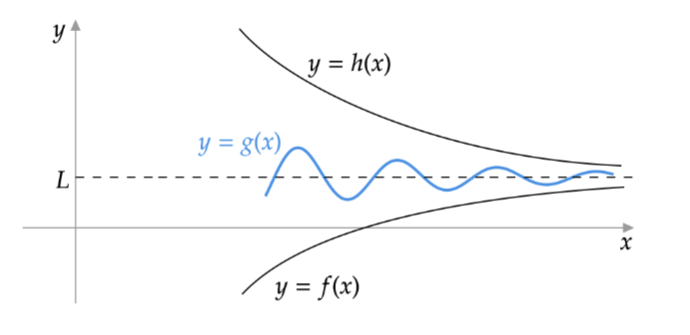
\includegraphics[width=0.8\textwidth]{images/pinching_theorem.png}
			\end{center}
		\end{figure}

		\begin{question}{Example}
			Find the limit of $g(x) = e^{-x^2} 2^{\sin{3x}}$ as $x \rightarrow \infty$ (if it exists).

			\begin{align*}
				& \sin{x} \in [-1,1], \quad \forall x \in \mathbb{R} \\
				& \Rightarrow \frac{1}{2} \leq 2^{\sin{3x}} \leq 2, \quad \forall x \in \mathbb{R} \\
				& \Rightarrow \frac{e^{-x^2}}{2} \leq e^{x^2} 2^{\sin{3x}} \leq 2e^{-x^2} \\
				\text{Since } & \lim_{x\to\infty} \frac{e^{-x^2}}{2} = \lim_{x\to\infty} 2e^{-x^2} = 0, \\
				& \therefore \lim_{x\to\infty} e^{-x^2} 2^{\sin{3x}} = 0
			\end{align*}
		\end{question}

	\subsection{Limits of the form $f(x)/g(x)$}

	When calculating $\displaystyle\lim_{x\to\infty} \frac{f(x)}{g(x)}$ when both $f(x)$ and $g(x)$ tend to $\infty$ as $x \rightarrow \infty$, the previous rules cannot be applied. The main goal in this situation is to \textbf{divide both $f$ and $g$ by the fastest growing term in $g$}.

	\begin{question}{Example}
		Find the limit $\displaystyle\lim_{x\to\infty} \frac{5x^3 + 6x^2 - 4 \sin{x}}{\cos{3x} + 5x - 2x^3}$ (if it exists).

		\begin{align*}
			\frac{5x^3 + 6x^2 - 4 \sin{x}}{\cos{3x} + 5x - 2x^3} &= \frac{5 + \frac{6}{x} - 4 \frac{\sin{x}}{x^3}}{\frac{\cos{3x}}{x^3} + \frac{5}{x^2} - 2}	\\
																 &= \frac{5 + 0 + 0}{0 + 0 - 2}	\\
																 &= -\frac{5}{2} \quad \text{ as } x \rightarrow \infty
		\end{align*}
	\end{question}

	\begin{question}{Example}
		Find the limit $\displaystyle\lim_{x\to\infty} \frac{x^2 + 3x}{\sqrt{2x^4 + 3} - 4x}$ (if it exists).

		\begin{align*}
			\frac{x^2 + 3x}{\sqrt{2x^4 + 3} - 4x} &= \frac{1 + \frac{3}{x}}{\frac{1}{x^2}\sqrt{2x^4 + 3} - \frac{4}{x}}	\\
												  &= \frac{1 + \frac{3}{x}}{\sqrt{2 + \frac{3}{x^4}} - \frac{4}{x}}	\\
												  & \rightarrow \frac{1 + 0}{\sqrt{2 + 0} - 0}	\\
												  &= \frac{1}{\sqrt{2}} \quad \text{as } x \rightarrow \infty
		\end{align*}
	\end{question}

	\subsection{Limits of the form $\sqrt{f(x)} - \sqrt{g(x)}$}

		In this case, the leading term may not help. Instead the lower order term will usually determine the limit. This can be achieved by \textbf{multiplying the numerator and denominator by the conjugate}.

		\begin{question}{Example}
			Find the limit of $\displaystyle\lim_{x\to\infty} \sqrt{2x^2 + 3x} - \sqrt{2x^2 - x}$.
			\begin{align*}
				\sqrt{2x^2 + 3x} - \sqrt{2x^2 - x} &= \frac{\left(\sqrt{2x^2 + 3x} - \sqrt{2x^2 - x} \right) \left(\sqrt{2x^2 + 3x} + \sqrt{2x^2 - x} \right)}{\left(\sqrt{2x^2 + 3x} + \sqrt{2x^2 - x} \right)}	\\
												   &= \frac{2x^2 + 3x - \left(2x^2 -x\right)}{\sqrt{2x^2 + 3x} + \sqrt{2x^2 -x}}	\\
												   &= \frac{4x}{\sqrt{2x^2 + 3x} + \sqrt{2x^2 - x}}	\\
												   &= \frac{x}{\sqrt{2 + \frac{3}{x}} + \sqrt{2 - \frac{1}{x}}}	\\
												   & \Rightarrow \frac{4}{\sqrt{2} + \sqrt{2}}	\\
												   &= \sqrt{2} \quad \text{as } x \rightarrow \infty
			\end{align*}
		\end{question}

	\subsection{Indeterminate forms}
		
		Some limits such as the form $\frac{\infty}{\infty}$ cannot be detemined in advance and is hence called an indeterminate form. Other indeterminate forms include:
		\begin{itemize}
			\item $\infty - \infty$ if $f(x) \rightarrow \infty$ and $g(x) \rightarrow \infty$ as $x \rightarrow \infty$, \quad $f(x) - g(x) \rightarrow ?$
			\item $\frac{0}{0}$ if $f(x) \rightarrow 0$ and $g(x) \rightarrow 0$ as $x \rightarrow \infty$, \quad $\frac{f(x)}{g(x)} \rightarrow ?$
			\item $0 \times \infty$ if $f(x) \rightarrow 0$ and $g(x) \rightarrow \infty$ as $x \rightarrow \infty$, \quad $f(x)g(x) \rightarrow ?$
		\end{itemize}

\section{The definition of $\displaystyle\lim_{x\to\infty} f(x)$}

	Suppose that $b, L \in \mathbb{R}$, and $f$ is a real-valued function defined on $(b, \infty)$. It is said:
		\begin{align*}
			\lim_{x\to\infty} f(x) = L
		\end{align*}
	if for every $\epsilon > 0$, there is $M \in \mathbb{R}$ such that:
		\begin{align*}
			x > M \Rightarrow |f(x) - L| < \epsilon
		\end{align*}

\section{Proving that $\displaystyle\lim_{x\to\infty} f(x) = L$ using the limit definition}

	\begin{question}{Example}
		Prove that $\displaystyle\lim_{x\to\infty} \frac{5x}{x+3} = 3$.
		\begin{alignat*}{2}
			& \left|f(x) - L\right| < \epsilon \text{ if ?}	\\
			& \left|f(x) - L\right| = \left|\frac{5x}{x+3} - 5 \right| = \left|\frac{5x - 5(x+3)}{x+2}\right| &&= \left|\frac{-15}{x+3}\right|	\\
			& && = \frac{15}{x+3} \quad \text{ for } x > 3	\\
			& && < \frac{15}{x} \quad \text{ for } x > 0	\\
			& \Rightarrow \left|f(x) - L\right| < \epsilon \quad \text{if} \quad \frac{15}{x} < \epsilon \text{ and } x > 0 	\\
			& \qquad (\text{i.e. } x > \frac{15}{\epsilon} > 0)	\\
			& \Rightarrow \text{For any } \epsilon > 0, \exists M = \frac{15}{\epsilon} \text{ such that }	\\
			& \qquad |f(x) - L| < \epsilon \text{ whenever } x > M
		\end{alignat*}
	\end{question}

	\subsubsection{Strategy for finding $M$}

		\begin{enumerate}
			\item Find a good upper bound for $|f(x) - L|$
			\item Find a simple condition on $x$ such that this upper bound is less than $\epsilon$
			\item Use this condition to state an appropriate value for M
		\end{enumerate}

		\textcolor{pastel_red}{Note:} The value of $M$ is not unique. If $M_0$ is a value for $M$, then any upper bound of $M_0$ is also a value for $M$

		\begin{question}{Example}
			Show that $\displaystyle\lim_{x\to\infty} \frac{x^2 - \cos{x}}{x^2 + 1} = 1$
			\begin{alignat*}{2}
				& \left| \frac{x^2 - \cos{x}}{x^2 + 1} - 1 \right| = \left| \frac{x^2 - \cos{x} - (x^2 + 1)}{x^2 + 1} \right| = \left| \frac{-\cos{x} - 1}{x^2 + 1} \right| &&= \left| \frac{\cos{x} + 1}{x^2 + 1} \right|	\\
				& && \leq \frac{2}{x^2 + 1}	\\
				& && \leq \frac{2}{x^2}	\\
				& \Rightarrow \left| f(x) - 1 \right| < \epsilon \quad \text{if} \quad \frac{2}{x^2} < \epsilon	\\
				& \qquad \because \frac{2}{x^2} < \epsilon \Leftrightarrow \sqrt{\frac{2}{\epsilon}} < x \quad \text{for} \quad x > 0, \quad M \triangleq \sqrt{\frac{2}{\epsilon}}
			\end{alignat*}
		\end{question}

\section{Proofs of basic limit results}
	
	Not assessable.

\section{Limits of functions at a point}
	
	\subsection{Left-hand, right-hand and two-sided limits}

		\begin{itemize}
			\item If $f(x)$ approaches $L$ as $x$ approaches $a$ from the \textcolor{pastel_blue}{left}-hand side, then:
				\begin{align*}
					\lim_{x\to a^-} f(x) = L \qquad \text{(left-hand limit)}
				\end{align*}
			\item If $f(x)$ gets arbitrarily large as $x$ approaches $a$ from the \textcolor{pastel_blue}{left} side, then:
				\begin{align*}
					f(x) \rightarrow \infty \quad \text{as} \quad x \rightarrow a^-
				\end{align*}
		\end{itemize}

		\begin{figure}[H]
			\begin{center}
				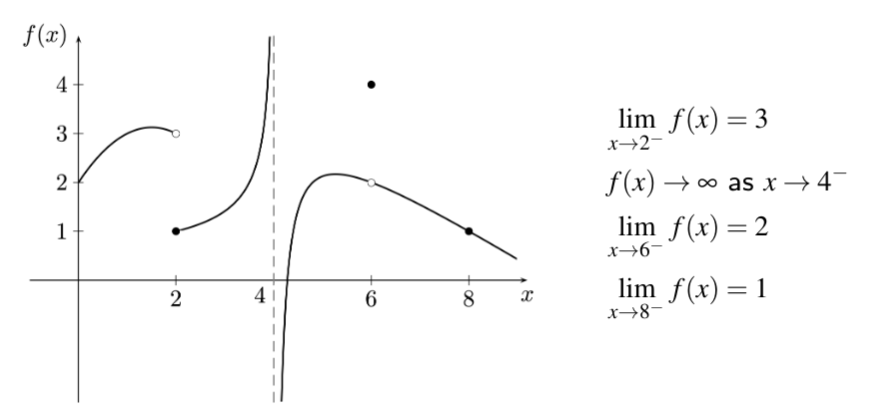
\includegraphics[width=0.8\textwidth]{images/left_hand_limits.png}
			\end{center}
		\end{figure}

		\begin{itemize}
			\item If $f(x)$ approaches $L$ as $x$ approaches $a$ from the \textcolor{pastel_blue}{right}-hand side, then:
				\begin{align*}
					\lim_{x\to a^+} f(x) = L \qquad \text{(right-hand limit)}
				\end{align*}
			\item If $f(x)$ gets arbitrarily large as $x$ approaches $a$ from the \textcolor{pastel_blue}{right} side, then:
				\begin{align*}
					f(x) \rightarrow \infty \quad \text{as} \quad x \rightarrow a^+
				\end{align*}
		\end{itemize}

		\begin{figure}[H]
			\begin{center}
				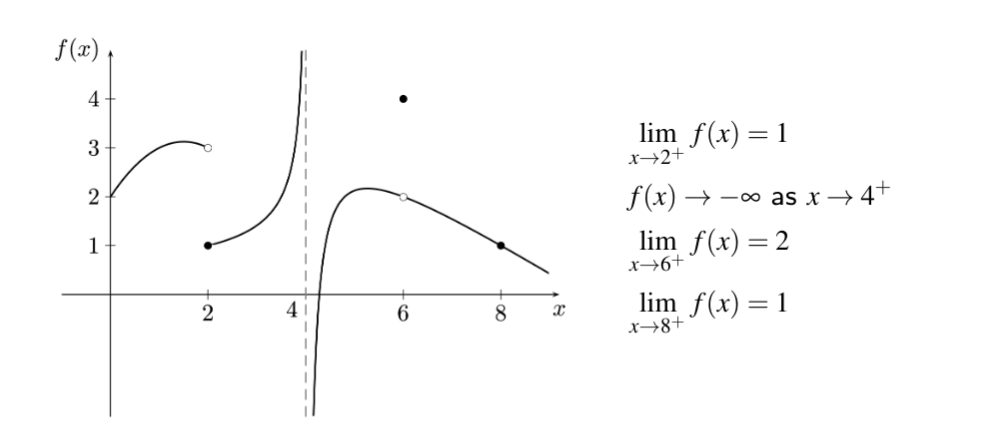
\includegraphics[width=0.8\textwidth]{images/right_hand_limits.png}
			\end{center}
		\end{figure}

		\begin{itemize}
			\item Left $I$ be an open interval that contains the point $a$. For a real-valued function $f$ defined on $I$ except possibly at $a$, if both one-sided limits exist and
				\begin{align*}
					\lim_{x\to a^-} f(x) = \lim_{x\to a^+} f(x) = L,
				\end{align*}
				then we say that thw (two-sided) limit of $f(x)$ as $x \rightarrow a$ exists and is equal to $L$, and we write
				\begin{align*}
					\lim_{x\to a} f(x) = L.
				\end{align*}
				Otherwise, $\displaystyle\lim_{x\to a} f(x)$ does not exist.
			\item \textcolor{pastel_red}{Note:} $f(a)$ is irrelevant to $\displaystyle\lim_{x\to a} f(x)$. $f$ does not need to be defined at $a$
		\end{itemize}

		\begin{figure}[H]
			\begin{center}
				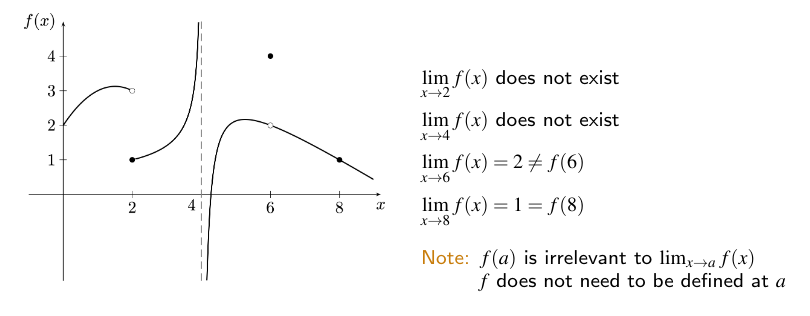
\includegraphics[width=0.8\textwidth]{images/two_sided_limits.png}
			\end{center}
		\end{figure}

	\subsection{Limits and continuous functions}

		Let $I$ be an open interval that contains the point $a$. A function $f: I \rightarrow \mathbb{R}$ is continuous at $a$ if
		\begin{align*}
			\lim_{x\to a} f(x) = f(a)
		\end{align*}
		Otherwise, we say that $f$ is discontinuous at $a$.
		\\
		\\
		If $f$ is continuous at every point of $\text{Dom}(f)$, then we say that $f$ is continuous everywhere.

		\begin{figure}[H]
			\begin{center}
				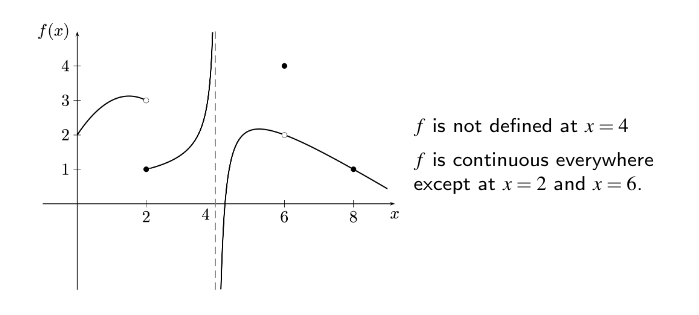
\includegraphics[width=0.8\textwidth]{images/continuity.png}
			\end{center}
		\end{figure}

	\subsection{Rules for limits at a point}
			
		\subsubsection{Arithmetic}

			Suppose that $a \in \mathbb{R}$, and $\displaystyle\lim_{x\to a} f(x) = L_1$ and $\displaystyle\lim_{x\to a} g(x) = L_2$. Then

			\begin{itemize}
				\item $\displaystyle\lim_{x\to a} (f(x) + g(x)) = L_1 + L_2$
				\item $\displaystyle\lim_{x\to a} (f(x) - g(x)) = L_1 - L_2$
				\item $\displaystyle\lim_{x\to a} f(x)g(x) = L_1 L_2$
				\item $\displaystyle\lim_{x\to a} \frac{f(x)}{g(x)} = \frac{L_1}{L_2}$
			\end{itemize}

		\subsubsection{Function composition}

				If $\displaystyle\lim_{x\to a} f(x) = L$ and $g$ is continuous at $L$, then

				\begin{align*}
					\lim_{x\to a} g(f(x)) = g\left(\lim_{x\to a} f(x)\right) = g(L)
				\end{align*}

			\begin{question}{Example}
				Find the limit $\displaystyle\lim_{x\to 5} \sqrt{2x + \cos{\pi x^2}}$.
				\begin{align*}
					\lim_{x\to 5} \sqrt{2x + \cos{\pi x^2}} &= \sqrt{\lim_{x\to 5} 2x + \cos{\pi x^2}} \qquad \left(\text{$\sqrt{\quad}$ is continuous} \right)	\\
															&= \sqrt{\lim_{x\to 5} 2x + \lim_{x\to 5} \cos{\pi x^2}}	\\
															&= \sqrt{\lim_{x\to 5} 2x + \cos{\lim_{x\to 5} \pi x^2}} \qquad \left(\text{cos is continuous} \right)\\
															&= \sqrt{10 + \cos{5^2 \pi}} \qquad \left(\cos{5^2 \pi} = -1 \right)	\\
															&= 3
				\end{align*}
			\end{question}

		\subsubsection{Pinching theorem (two-sided limit)}

			Let $I$ be an open interval that contains the point $a$. Suppose that $f$, $g$, and $h$ are functions defined on $I$. If
			\begin{itemize}
				\item $f(x) \leq g(x) \leq h(x), \quad \forall x \in I$, and
				\item $\displaystyle\lim_{x\to a} f(x) = \displaystyle\lim_{x\to a} h(x) = L$
			\end{itemize}
			then
			\begin{align*}
				\lim_{x\to a} g(x) = L
			\end{align*}

			\begin{figure}[H]
				\begin{center}
					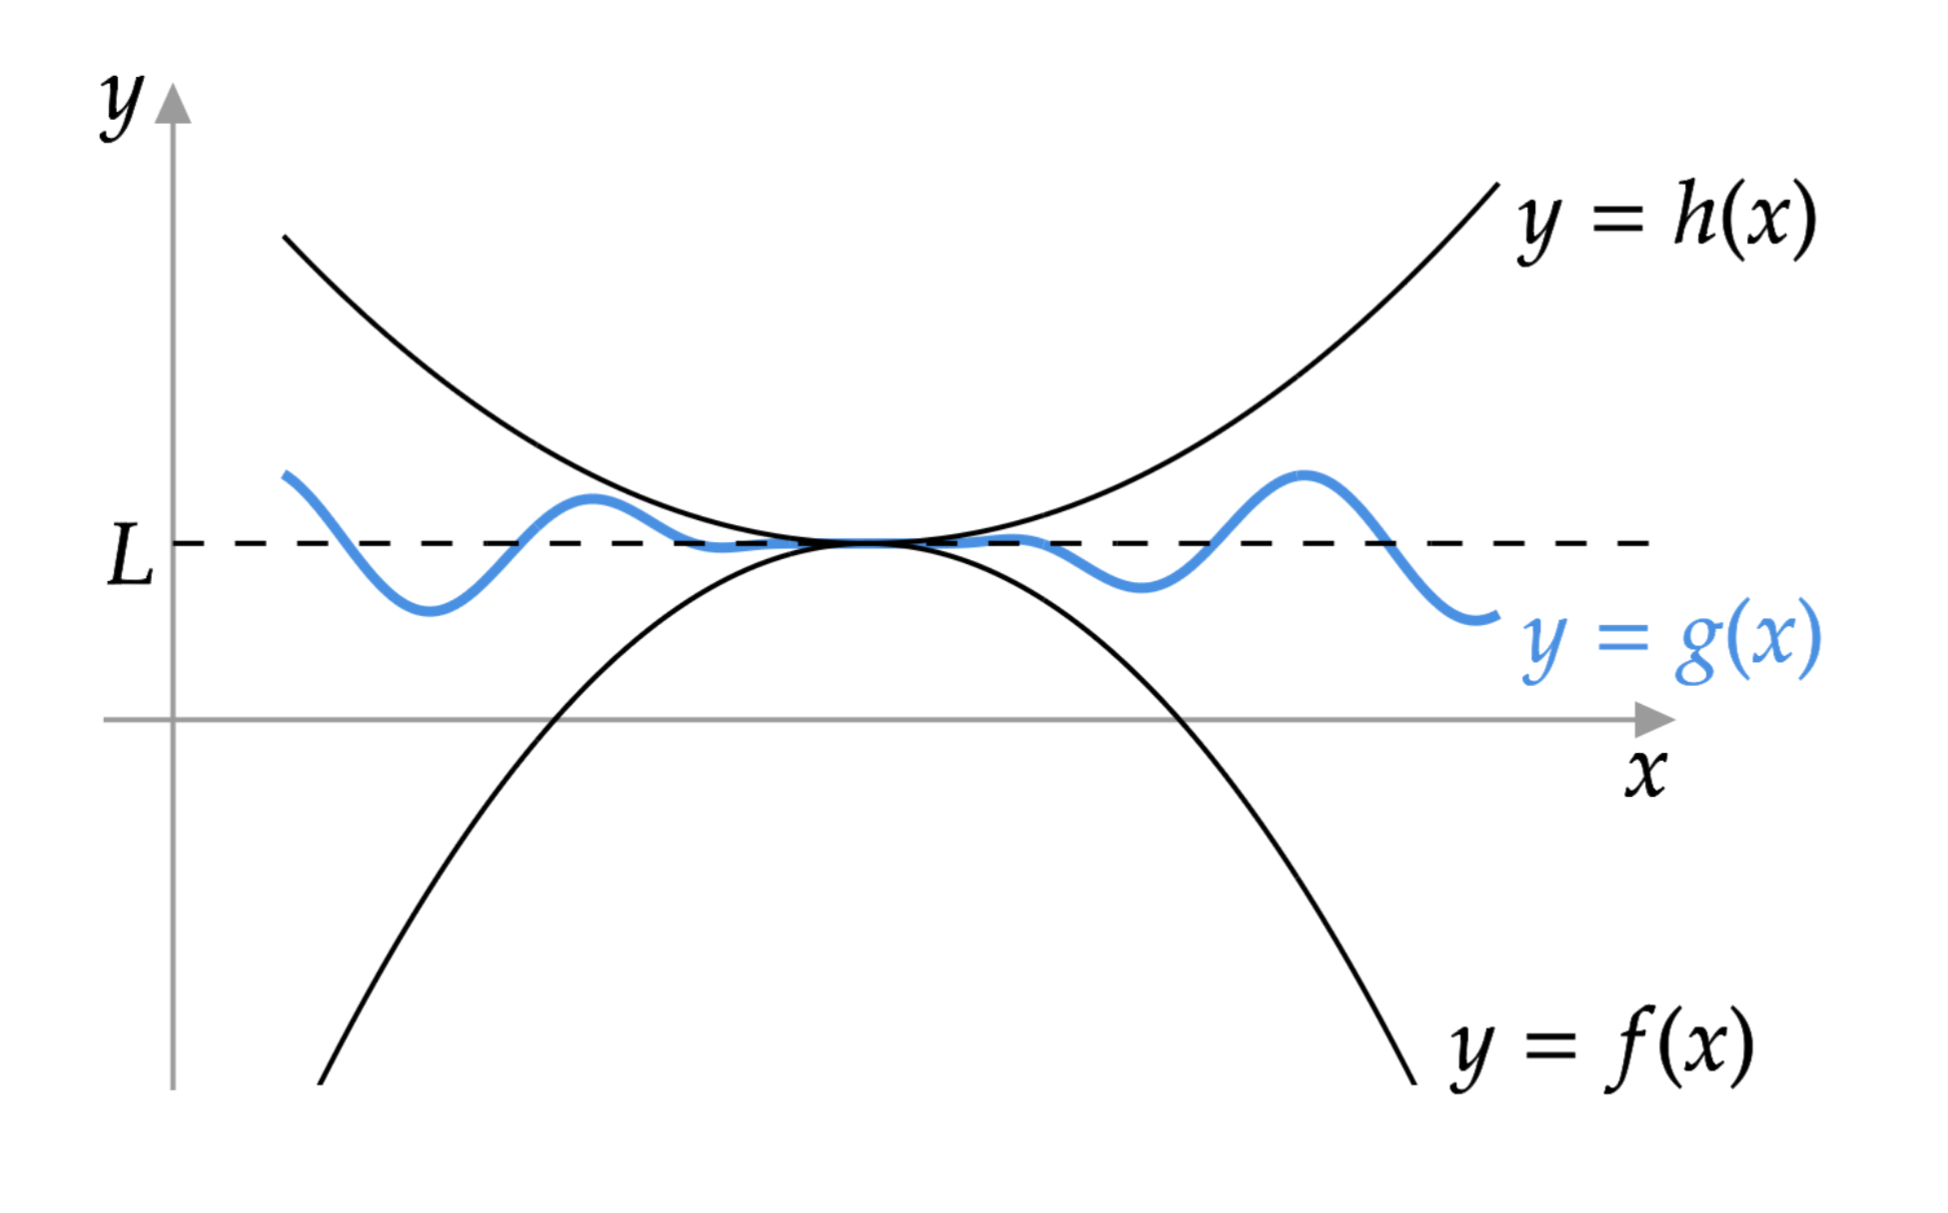
\includegraphics[width=0.8\textwidth]{images/two_sided_pinching_theorem.png}
				\end{center}
			\end{figure}

			\begin{question}{Example}
				Suppose that $f: \mathbb{R} \rightarrow \mathbb{R}$ is defined by the formula
				\begin{align*}
					f(x) = \begin{cases}
						\frac{|x^2 - 9|}{x-3} \qquad & \text{if } x \neq 3\\
						-6 &\text{if } x = 3
					\end{cases}
				\end{align*}

				Discuss the limiting behaviour of $f(x)$ as $x$ approaches 3.
				\\
				\\
				Limit from left hand side
				\begin{alignat*}{2}
					& \text{For } x \in (-3,3), \qquad && \frac{|x^2 -9|}{x-3} = \frac{|x+3||x-3|}{x-3} = -(x+3)	\\
					&								  && \Rightarrow \lim_{x\to 3^-} f(x) = \lim_{x\to 3^-} -(x+3) = -6 = f(3)
				\end{alignat*}

				Limit from right hand side
				\begin{align*}
					\text{For } x > 3, & \qquad \frac{|x^2 -9|}{x-3} = x+3	\\
									   & \qquad \Rightarrow \lim_{x\to 3^+} f(x) = \lim_{x\to 3^+} x+3 = 6
				\end{align*}
				Since $\displaystyle\lim_{x\to 3^+} f(x) \neq \lim_{x\to 3^-} f(x)$, two-sided limit does not exist at $x = 3$

				So, $f$ is not continuous at $x = 3$

			\end{question}

\chapter{Properties of continuous functions}

\section{Combining continuous functions}
	
	Suppose that the functions $f$ and $g$ are continuous at a point $a$. Then
	\begin{enumerate}
		\item $f+g$, $f-g$ and $fg$ are continuous at $a$
		\item $\frac{f}{g}$ is continuous at $a$, provided that $g(a) \neq 0$
	\end{enumerate}
	\begin{alignat*}{2}
		\lim_{x\to a} (f+g)(x) &= \lim_{x\to a} (f(x) + g(x)) \qquad \qquad 	&& (\text{by definition of } f+g)	\\
							   &= \lim_{x\to a} f(x) + \lim_{x\to a} g(x) 		&& (\text{by "limit of sum = sum of limits"})	\\
							   &= f(a) + g(a)									&& (\text{by continuity of } f \text{ and } g \text{ at } a)	\\
							   &= (f+g)(a)
	\end{alignat*}

	Supose that the function $f$ is continuous at $a$, and $g$ is continuous at $f(a)$. Then $g \circ g$ is continuous at $a$.
	\begin{alignat*}{2}
		\lim_{x \to a} (g \circ f)(x) &= \lim_{x \to a} g(f(x)) \\
									  &= g\!\left( \lim_{x \to a} f(x) \right) \qquad \qquad	&& (\text{by limit rule of function composition}) \\
									  &= g(f(a))												&& (\text{by continuity of $f$ at $a$}) \\
									  &= (g \circ f)(a)
	\end{alignat*}

	\begin{question}{Example}
		Every polynomial $p: \mathbb{R} \rightarrow \mathbb{R}$ is continuous at every $a \in \mathbb{R}$.
		\begin{align*}
			\Leftarrow \text{for any } n \in \mathbb{N}, \quad p(x) &= a_n x^n + a_{n-1} x^{n-1} + \dots + a_0	\\
																	&= \text{product \& sum of } g(x) = x \text{ and contant functions, ie. continuous by (i)}
		\end{align*}
	\end{question}

\section{Continuity on intervals}

	For a real-valued function $f$ defined on an open interval $(a,b)$, we say that $f$ is continuous on $(a,b)$ if it is continuous at every $x \in (a,b)$.

	For a real-valued function $f$ defined on a closed interval $[a,b]$, we say that
		\begin{itemize}
			\item $f$ is continuous at the endpoint $a$ if $\displaystyle\lim_{x\to a^+} f(x) = f(a)$
			\item $f$ is continuous at the endpoint $b$ if $\displaystyle\lim_{x\to b^-} f(x) = f(b)$
			\item $f$ is continuous on $[a,b]$ if it is continuous on $(a,b)$ and at endpoints $a$ and $b$.
		\end{itemize}

\section{The intermediate value theorem}

	Suppose that $f$ is continuous on $[a,b]$, and $f(b) < z < f(a)$ for some $z$. The graph of $f$ from $(a, f(a))$ to $(b, f(b))$ without lifting the pen. We must cross a point $(c,z)$ along the way for some $c \in (a,b)$.

	Let $f: [a,b] \rightarrow \mathbb{R}$ be a continuous function. If either $f(a) < z < f(b)$ or $f(b) < z < f(a)$ for some $z \in \mathbb{R}$, then there is at least one $c \in (a,b)$ such that $f(c) = z$

	\begin{itemize}
		\item In general, $c$ is not unique
		\item The continuity of $f$ is necessary
		\item Only for continuous functions defined on (subsets of) $\mathbb{R}$, no analogue for $\mathbb{Q}$
			\begin{alignat*}{2}
				& f: \mathbb{R} \rightarrow \mathbb{R}, \quad f(x) = x^2 - 2 \qquad && f \text{ is continuous on Dom}(f) = \mathbb{R}	\\
				&																	&& = \in \left(f(0),f(2)\right),\;f(c) = 0 \text{ at } c = \sqrt{2} \in (0,2)	\\
				& f: \mathbb{Q} \rightarrow \mathbb{Q}, \quad g(x) = x^2 - 2 \qquad && g \text{ is continuous on Dom}(g) = \mathbb{Q}	\\
				&																	&& = \in \left(g(0),g(2)\right),\;g(c) = 0 \text{ at } c = \sqrt{2} \notin \mathbb{Q}	\\
			\end{alignat*}
		\item Since infinity is not part of $\mathbb{R}$, a definite bound must be defined before using IVT
	\end{itemize}

	\begin{question}{Example}
		Show that there exists a solution $c \in [1,2]$ of the equation $\sqrt{c} = c^2 - 1$ and approximate its value.
		\\ \\
		Define a function $f: [1,2] \rightarrow \mathbb{R}$ by $f(x) = x^2 - 1 - \sqrt{x}$. Then,
			\begin{itemize}
				\item $f$ is continuous on [1,2]
				\item $f(1) = -1$  and $f(2) = 3 - \sqrt{2} > 0$.
			\end{itemize}

		Since $f(1) < 0 < f(2)$, by \textcolor{pastel_orange}{IVT}, there is a number $c \in (1,2)$ such that $f(c) = c^2 - 1 - \sqrt{c} = 0$
		\\ \\
		Approximation:
		\begin{itemize}
			\item take $c_1 = 1.5 \Rightarrow f(c_1) = 0.0253$, by IVT, $\exists$ a solution $c \in (1, c_1)$
			\item take $c_2 = 1.25 \Rightarrow f(c_2) = -0.5555$, by IVT, $\exists$ a solution $c \in (1, c_2)$
		\end{itemize}

	\end{question}

\section{The maximum-minimum theorem}

	Let $f$ be a real-valued function defined on a closed interval $[a,b]$.
	\begin{itemize}
		\item A point $c \in [a,b]$ is a global minimum point for $f$ on $[a,b]$ if
			\begin{align*}
				f(c) \leq f(x), \quad \forall x \in [a,b].
			\end{align*}
		\item A point $d \in [a,b]$ is a global minimum point for $f$ on $[a,b]$ if
			\begin{align*}
				f(d) \geq f(x), \quad \forall x \in [a,b].
			\end{align*}
	\end{itemize}

	If $f$ is continuous on $[a,b]$, then $f$ attains its minimum and maximum on $[a,b]$, ie. there exists points $c,d \in [a,b]$ such that
		\begin{align*}
			f(c) \leq f(x) \leq f(d), \quad \forall x \in [a,b].
		\end{align*}

	\begin{itemize}
		\item Closed intervals are necessary
		\item Continuity of $f$ is necessary
	\end{itemize}

	\begin{question}{Example}
		Let $f$ be a function defined by $f(x) = \begin{cases} \frac{1}{x^2+1} \sin{\frac{1}{x}}, \quad & \text{ if } x \neq 0 \\	1, & \text{ if } x=0 \end{cases}$

		\begin{enumerate}
			\item Is $f$ bounded on $[-2,2]$?
				\begin{align*}
					\text{Yes. } \quad & \text{For } x \neq 0, \quad \left|f(x)\right| = \left| \frac{1}{x^2 + 1} \sin{\frac{1}{x}} \right| \leq \frac{1}{x^2 _ 1} \leq 1.	\\
									   & \text{For } x = 0, \quad f(x) = 1.	\\
									   & \Rightarrow \left|f(x)\right| \leq 1, \quad \forall \; x \in [-2,2]
				\end{align*}
			\item Does it attain a minimum or maximum on $[-2,2]$
				\begin{itemize}
					\item $f$ on $[-2,2]$ attains a maximum at $x=0$.
					\item $f$ does not have a minimum value on $[-2,2]$
				\end{itemize}
				\begin{align*}
					& \text{For } x_n = \left(\frac{-\pi}{2} + 2n \pi\right)^{-1}, \quad n \in \mathbb{Z}	\\
					& \qquad \sin{\frac{1}{x_n}} = -1	\\
					& \qquad f(x_n) = - \frac{1}{\left(\frac{- \pi}{2} + 2n \pi\right)^{-2} + 1}	\\
					& \text{Then as } n \rightarrow \infty, \quad x_n \rightarrow 0 \text{ and } f(x_n) \rightarrow -1	\\
					& \text{Note: } f(x) > -1	\\
					& \Rightarrow \text{as } x \rightarrow 0, f(x) \text{ oscillates between (not touching) } -1 \text{ and } 1
				\end{align*}
		\end{enumerate}
	\end{question}

\chapter{Differentiable functions}

	\section{Gradients of tangents and derivatives}

		Suppose that $f$ is defined on some open interval containing the point $x$. It is said that $f$ is differentiable at $x$ if

			\begin{align*}
				\lim_{h\to 0} \frac{f(x + h) - f(x)}{h} \quad \text{exists}
			\end{align*}

		This limit is denoted by $f'(x)$, $\frac{df}{dx} (x)$ or $\frac{d}{dx} f(x)$ and is called the derivative of $f$ at $x$.

		\begin{question}{Example}
			\begin{enumerate}
				\item Show that $\displaystyle\lim_{h\to 0} \frac{\cos(h) - 1}{h} = 0$. \quad (Hint: $\cos(h) - 1 = \frac{\cos^2 (h) - 1}{\cos (h) + 1} = -\frac{\sin^2 (h)}{\cos (h) + 1}$)
					\begin{align*}
						\lim_{h\to 0} \frac{\cos (h) - 1}{h} &= - \lim_{h\to 0} \frac{\sin(h)}{\cos(h) + 1} \frac{\sin(h)}{h}	\\
															 &= - \frac{\displaystyle\lim_{h\to 0} \sin(h)}{\displaystyle\lim_{h\to 0} \cos(h) + 1} \lim_{h\to 0} \frac{\sin(h)}{h} \qquad \left(\lim_{h\to 0} \frac{\sin(h)}{h} = 1\right)	\\
															 &= - \frac{0}{2} \times 1 = 0
					\end{align*}
				\item For which $n \in \mathbb{N}$ is the function $f$ defined by
					\begin{align*}
						f(x) = \begin{cases} x^n \sin\left(\frac{1}{x}\right) \quad & \text{if } x \neq 0	\\	0 & \text{if } x = 0 \end{cases}
					\end{align*}
					continuous and differentiable at $x = 0$
					\\ \\

					For continuity, $\displaystyle\lim_{x\to 0} x^n \sin\left(\frac{1}{x}\right) = f(0) = 0$.
					\begin{alignat*}
						-1 \leq \sin \left(\frac{1}{x}\right) \leq 1, \; \forall x\neq 0 \quad &\Rightarrow \quad -|x^n| \leq x^n \sin \left(\frac{1}{x}\right) \leq |x^n|, \; \forall x \neq 0, \; \forall n \in \mathbb{N}	\\
						\text{(Pinching theorem)} \quad &\Rightarrow \quad \lim_{x\to 0} x^n \sin\left(\frac{1}{x}\right) = 0, \quad \text{ie. continuous at } x=0,\; \forall n \in \mathbb{N} \textbackslash \{0\}
					\end{alignat*}

					For differentiability, $\displaystyle\lim_{h\to 0} \frac{1}{h} \left[f(0+h) - f(0) \right]$ exists.
					\begin{align*}
						&= \frac{1}{h} \left[ h^n \sin\left(\frac{1}{h}\right) - 0 \right]	\\
						&= h^{n-1} \sin \left(\frac{1}{h}\right) \rightarrow 0, \quad \forall n-1 \in \mathbb{N} \textbackslash \{0\}
					\end{align*}
					ie. $n \in \mathbb{N}, \; n \neq 0, 1$
			\end{enumerate}
		\end{question}

	\section{Rules for differentiation}
			
		Suppose that $f$ and $g$ are differentiable at $x$. Then $f+g$, $f-g$ and $fg$ are differentiable at $x$, and $\frac{f}{g}$ is also differentiable at $x$, provided $g(x) \neq 0$.

			\begin{enumerate}
				\item $(f+g)'(x) = f'(x) + g'(x)$
				\item $(Cf)'(x) = Cf'(x)$ where $C$ is any constant
				\item $(fg)'(x) = f'(x)g(x) + f(x)g'(x)$, (product rule)
				\item $\left(\frac{f}{g}\right)'(x) = \frac{f'(x)g(x) - f(x)g'(x)}{(g(x))^2}$, provided that $g(x) \neq 0$ (quotient rule)
			\end{enumerate}

		Suppose that $g$ is differentiable at $x$, and $f$ is differentiable at the point $g(x)$. Then $f \circ g$ is differentiable at $x$ and
		
		\begin{align*}
			(f \circ g)'(x) = f'(g(x))g'(x)
		\end{align*}

	\section{Proofs of results}
		
		lol no

	\section{Implicit differentiation}

		A function defined by an equation relating $x$ and $y$ is implicitly defined.

		\begin{question}{Example}
			Determine the tangent to the curve $x^4 - x^2 y^2 + y^4 = 13$ at $(2,1)$

			\begin{flalign*}
				y \text{ depends on } x: & y(x)		&\\
										 & \text{ in a neighbourhood of } (2,1)
			\end{flalign*}
			\begin{flalign*}
				& \text{Differentiate both sides of the equation with respect to x: }	&\\
				& \qquad 4x^3 - 2xy^2(x) - 2x^2 y(x) y'(x) + 4y^3(x)y'(x) = 0
			\end{flalign*}

			At $(x,y) = (2,1)$,
			\begin{flalign*}
				\qquad 32 - 4 - 8y'(2) + 4y'(2) &= 0	&\\
				28 - 4y'(2) &= 0						&\\
				y'(2) &= 7								&\\
			\end{flalign*}

			Tangent line at $(2,1)$:
			\begin{flalign*}
				& \qquad y - 1 = 7(x - 2)		&
			\end{flalign*}
		\end{question}

	\section{Differentiation, continuity and split functions}
		
		\begin{itemize}
			\item If $f$ is differentiable at $a$, then $f$ is continuous at $a$
			\item If $f$ is not continuous at $a$, then it is not differentiable at $a$
			\item If $f$ is continuous at $a$, it may not be differentiable at $a$
				\begin{itemize}
					\item eg. $f: \mathbb{R} \rightarrow \mathbb{R}, \; f(x) = |x|$ and $a=0$
				\end{itemize}
		\end{itemize}

		Suppose $a \in \mathbb{R}$ and the function $f$ is defined by 
		\begin{align*}
			f(x) = \begin{cases} p(x) \quad & \text{if } x \geq a	\\ q(x) & \text{if } x < a \end{cases}
		\end{align*}
		where $p$ and $q$ are differentiable in some open interval containing $a$. If
		
		\begin{itemize}
			\item $f$ is continuous at $a$ ($\Leftrightarrow p(a) = q(a)) and
			\item $p'(a) = q'(a)$,
		\end{itemize}

		then $f$ is differentiable at $x = a$.

	\section{Derivatives and function approximation}

		If $f$ is differentiable at $a$, then
		\begin{align*}
			f'(a) = \lim_{x\to a} \frac{f(x) - f(a)}{x-a}
		\end{align*}
		By the definition of a limit, $\frac{f(x) - f(a)}{x-a}$ gets close to $f'(a)$ as $x$ gets close to $a$. This statement is equivalent to
		\begin{align*}
			\frac{f(x) - f(a)}{x-a} \approx f'(a)	\\
			f(x) \approx f(a) + f'(a)(x-a)
		\end{align*}

		\begin{question}{Example}
			Estimate $\sin(0.51 \pi)$
			\begin{alignat*}{2}
				& \sin(0.51 \pi) &&\approx \sin(0.5 \pi) + \cos(0.5 \pi)(0.51 \pi - 0.5 \pi)	\\
				& &&= 1 + 0 \times (0.01 \pi)	\\
				& &&= 1		\\
				&\Rightarrow \sin(0.51 \pi) &&\approx 1
			\end{alignat*}
		\end{question}

	\section{Derivatives and rates of change}

		ext 1 content

	\section{Local maximum, local minimum and stationary points}

		Let $f$ be defined on some interval $I$.
		\begin{itemize}
			\item A point $c \in I$ is a local minimum if there exists a $h > 0$ such that
				\begin{align*}
					f(x) \geq f(c), \; x \in (c-h, c+h) \cap I
				\end{align*}
			\item A point $d \in I$ is a local maximum point if there exists a $h > 0$ such that
				\begin{align*}
					f(x) \leq f(d), \; x \in (d-h, d+h) \cap I
				\end{align*}
		\end{itemize}

\chapter{The mean value theorem and applications}

	\section{The mean value theorem}

		Suppose that $f$ is
		\begin{enumerate}
			\item continuous on $[a,b]$, and
			\item differentiable on $(a,b)$
		\end{enumerate}

		Then there is at least one $c \in (a,b)$ such that
		\begin{align*}
			\frac{f(b) - f(a)}{b-a} = f'(c)
		\end{align*}

		The mean value theorem cannot be applied if
		\begin{itemize}
			\item $f$ is not continuous on $[a,b]$
			\item $f$ is not differentiable on $(a,b)$
		\end{itemize}

		\begin{figure}[H]
			\centering
			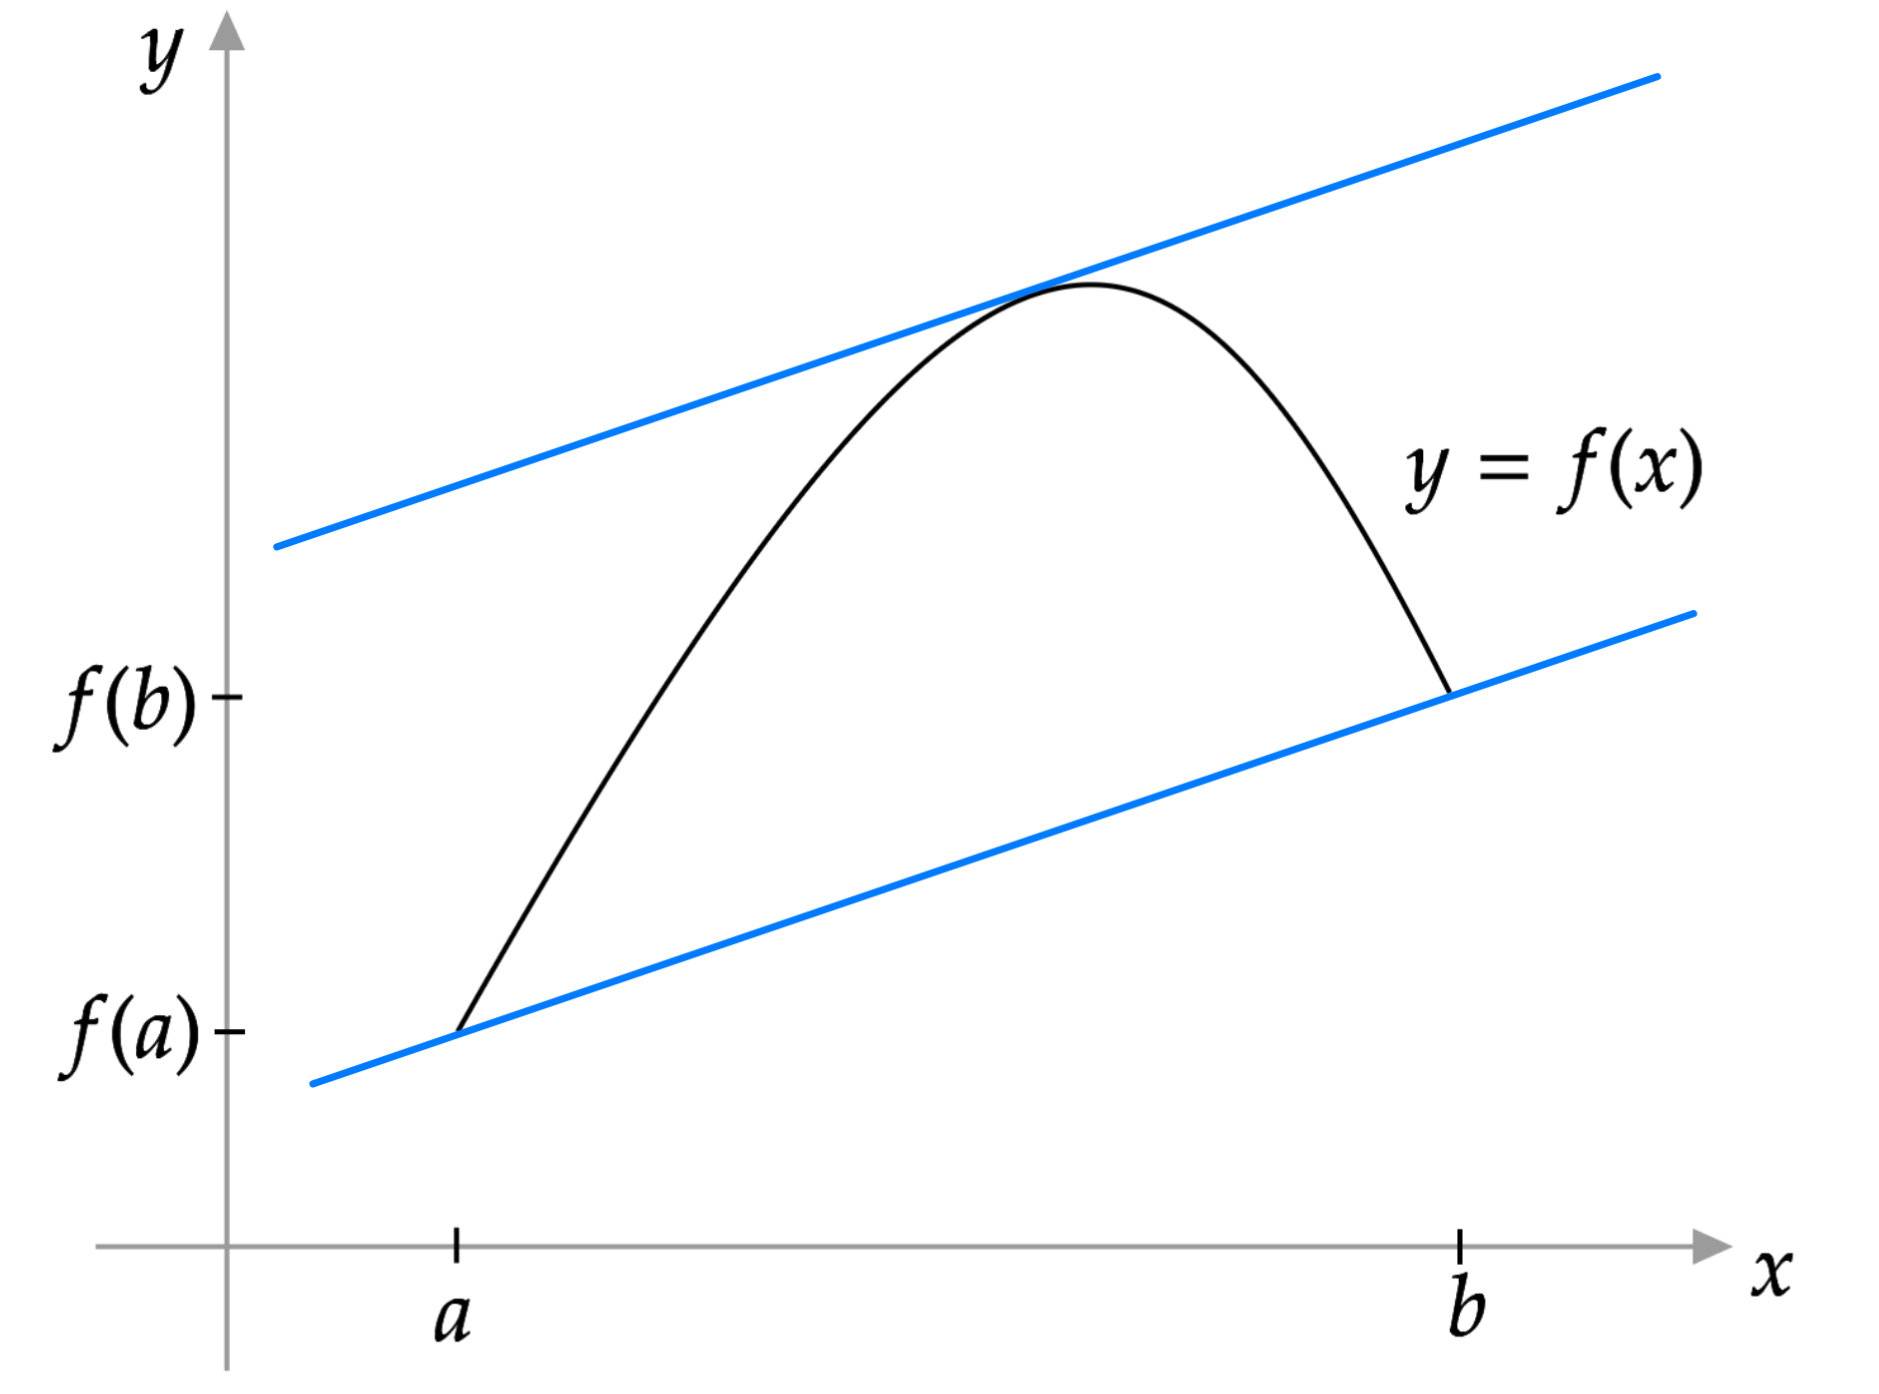
\includegraphics[width=0.7\textwidth]{images/mean_value.png}
		\end{figure}

		\begin{question}{Example}
			A car enters a tunnel at a speed of 30km/h and after 1 minute leaves the tunnel at a speed of 40km/h. The length of the tunnel is 1km. Did the driver break thespeed limit of 50km/h?
			\\ \\
			Let $x: [t_{in}, t_{out}] \rightarrow \mathbb{R}, \; x(t) = \text{ position of the car at time }t$

			Assume $x$ is continuous on $[t_{in}, t_{out}]$ and differentiable on $(t_{in}, t_{out})$

			$\Rightarrow$ By MVT, $\exists T \in (t_{in}, t_{out})$ such that
			\begin{align*}
				x'(t) = \frac{x(t_{out}) - x(t_{in})}{t_{out} - t_{in}} = \frac{1}{\frac{1}{60}} \text{km/h} = 60 \text{km/h}
			\end{align*}
			Therefore, the driver broke the speed limit
		\end{question}

	\section{Proof of the mean value theorem}

		Suppose that $g$
		\begin{itemize}
			\item is continuous on $[a,b]$
			\item differentiable on $(a,b)$
			\item $g(a) = g(b) = 0$ (optional)
		\end{itemize}
		Then there is $c \in (a,b)$ such that $g'(c) = 0$

		\begin{question}{Proof of Rolle's theorem}

			\begin{figure}[H]
				\centering
				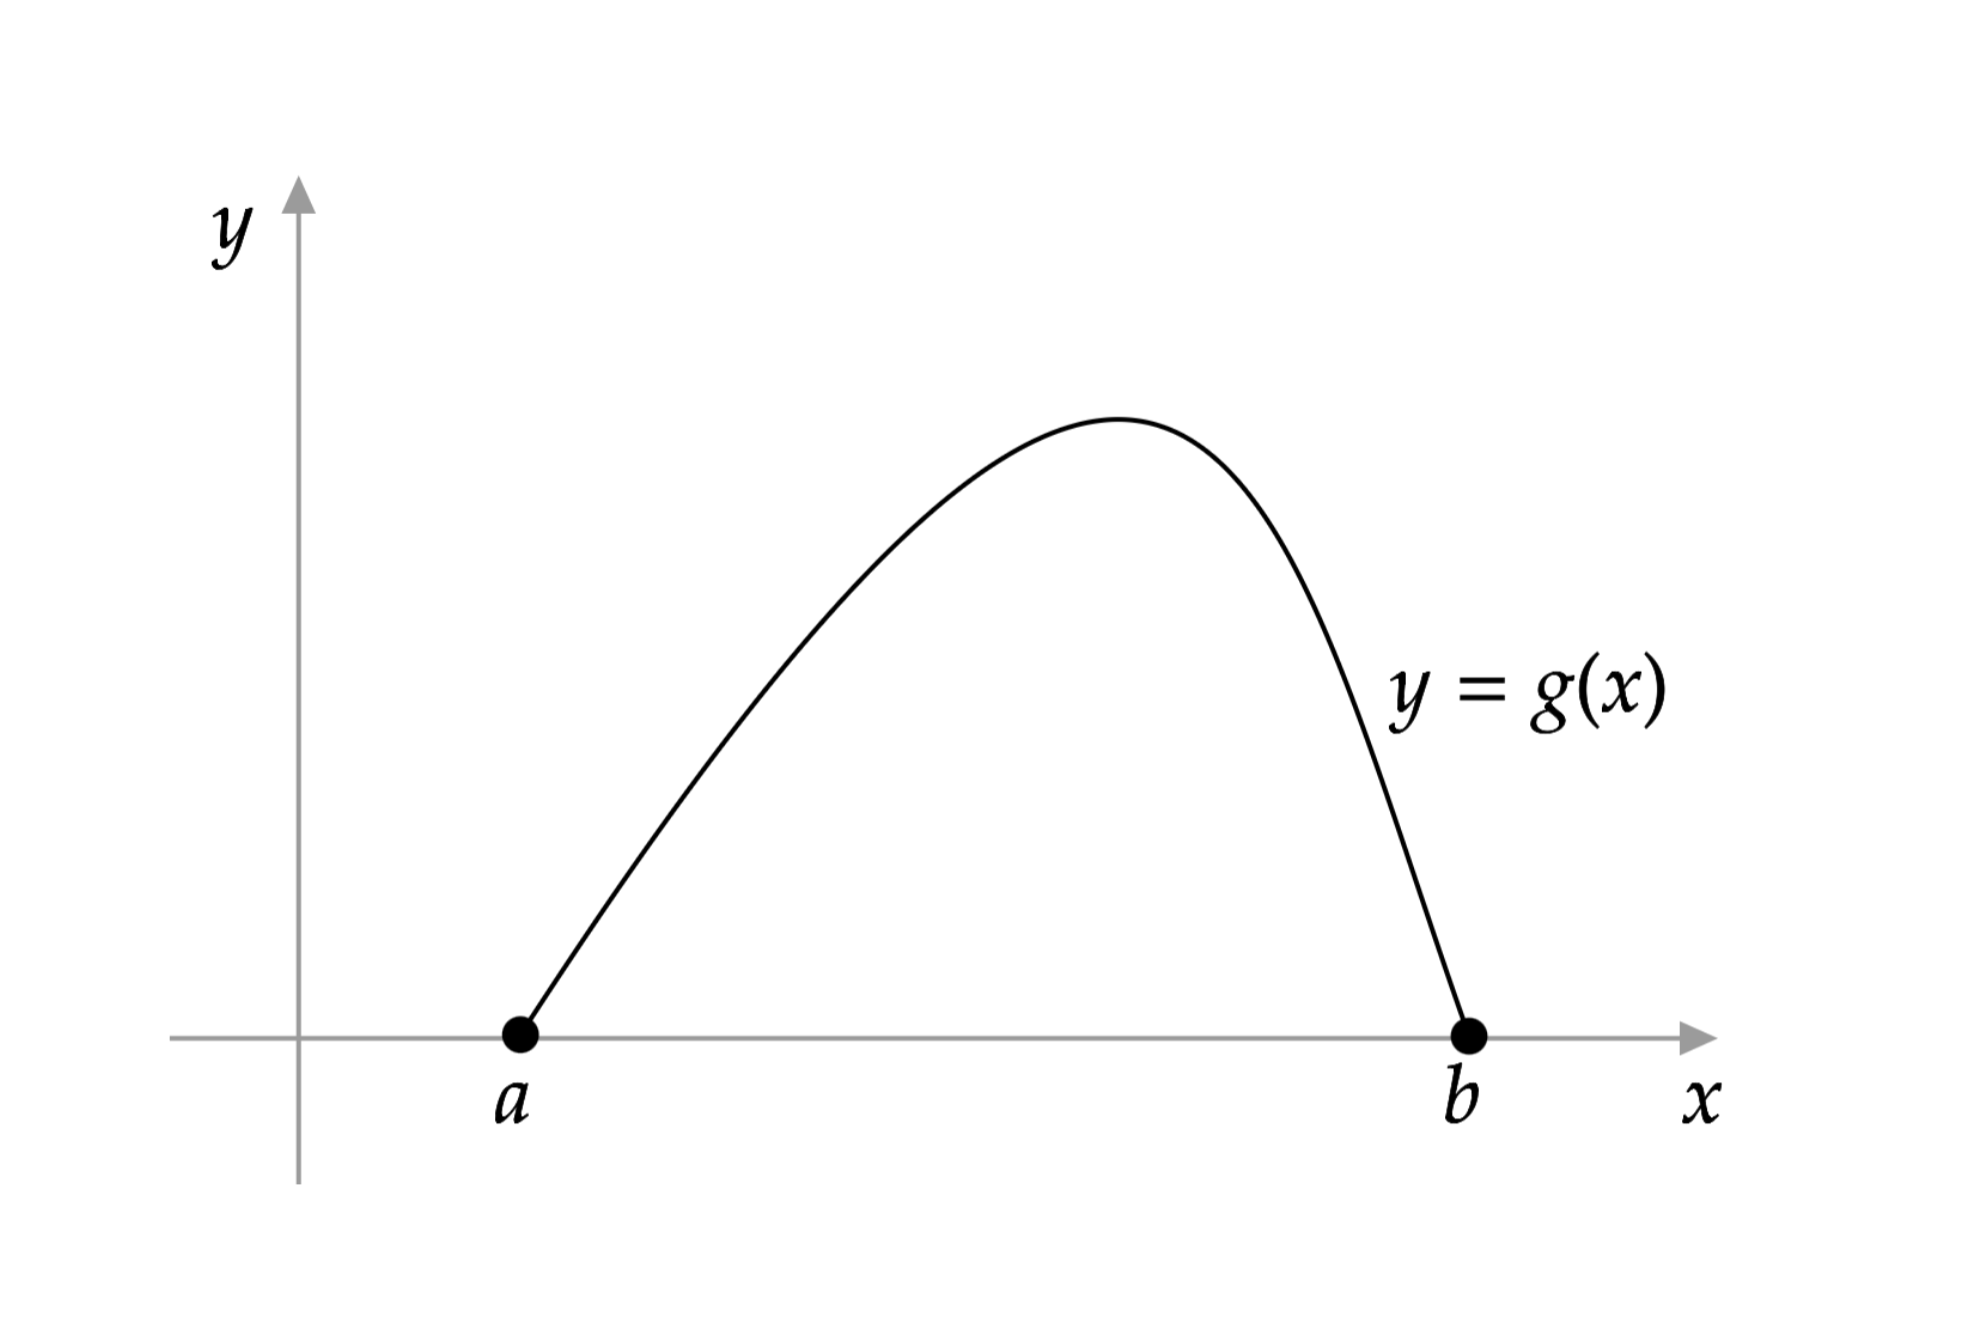
\includegraphics[width=0.7\textwidth]{images/rolles.png}
			\end{figure}

			\textbf{Case 1}: $g(x) = 0, \;\forall x \in [a,b]$

			\quad $\Rightarrow g'(c) = 0$ for any $c \in (a,b)$
			\\ \\
			\textbf{Case 2}: $g(d) > 0$ for some $d \in (a,b)$

			\quad By continuity and MMT, $g$ attains a maxmimum value at some $c \in [a,b]$
			\begin{flalign*}
				\quad \text{Then } & g(c) \geq g(d) > 0 = g(a) = g(b)	&\\
							& \Rightarrow c \neq a, c \neq b, \text{ so } c \in (a,b)	&\\
							& \Rightarrow g'(c) = 0
			\end{flalign*}
	
			\textbf{Case 3:} $g(x) \leq 0, \; \forall x \in [a,b]$, and $g$ is not a constant on $[a,b]$

			\quad Since $g(a) = g(b)$, Case 3 $\Leftrightarrow g(d) < 0$ for some $d \in (a,b)$

			\quad Similar to Case 2, $g$ attains a minimum value atsome $c \in (a,b)$, $g'(c) = 0$

		\end{question}

		\\ \\
		To prove MVT, a function $f$ is "deformed" such that it looks like $g$ in Rolle's theorem.
		\begin{flalign*}
			\text{Define } g: & [a,b] \rightarrow \mathbb{R} \text{ by}		&\\
							  & g(x) = f(x) - \frac{f(b) - f(a)}{b-a} x		&\\
		\end{flalign*}
		Hence
		\begin{flalign*}
			\exists c \in (a,b) \text{ such that } g'(c) = 0 \quad \Leftrightarrow \quad f'(c) - \frac{f(b) - f(a)}{b-a} = 0
		\end{flalign*}

	\section{Proving inequalities using the mean value theorem}

		From the equality $\frac{f(b) - f(a)}{b-a} = f'(c)$ in MVT,
		\begin{align*}
			m \leq f'(c) \leq M \quad \Longleftrightarrow \quad m \leq \frac{f(b) - f(a)}{b-a} \leq M
		\end{align*}

		\begin{question}{Example}
			Use MVT to show that $e^x > 1+x$ for all $x > 0$
			\\ \\
			For any $x > 0$, define a function
			\begin{align*}
				f: [0,x] \rightarrow \mathbb{R}, \quad f(t) = e^t
			\end{align*}
			\begin{itemize}
				\item $f$ is continuous on $[0,x]$
				\item $f$ is differentiable on $(0,x)$
			\end{itemize}
			\begin{flalign*}
				\text{Hence, by MVT, } \exists c \in (0,x) \text{ such that } \frac{f(x) - f(0)}{x - 0} &= f'(c)	&\\
																										& \Updownarrow	&\\
										\frac{e^x - 1}{x} &= e^c > 1	&\\
										e^x - 1 &> x	&\\
										e^x &> 1+x
			\end{flalign*}
		\end{question}

		\begin{question}{Example}
			Use MVT to show that $\ln (x) < x-1$ for all $x > 1$
			\\ \\
			For any $x > 1$, define a function
			\begin{align*}
				f: [1,x] \rightarrow \mathbb{R}, \; f(t) = \ln(t)
			\end{align*}

			\begin{flalign*}
				\text{By MVT, } \exists c \in (1,x) \text{ such that } \frac{f(x) - f(1)}{x-1} &= f'(c)	&\\
																							   &\Updownarrow	&\\
																		\frac{\ln(x) - 0}{x-1} & = \frac{1}{c} < 1	&\\
																						\ln(x) &< x-1	&
			\end{flalign*}
		\end{question}

	\section{Error bounds}

		From the equality $\frac{f(b) - f(a)}{b-a} = f'(c)$ in MVT,
		\begin{align*}
			|f(b) - f(a)| \leq M \quad \Longleftrightarrow \quad |f'(c)||b-a| \leq M
		\end{align*}

		\begin{question}{Example}
			How good an approximation of $\cos 1$ is $\cos \frac{\pi}{3}$

			By MVT, $\exists c \in \left(1, \frac{\pi}{3}\right)$ such that
			\begin{align*}
				\frac{\cos(1) - \cos\left(\frac{\pi}{3}\right)}{1 - \frac{\pi}{3}} = f'(c) = -\sin(c)
			\end{align*}
			\begin{alignat*}{2}
				&\Rightarrow 0 < \cos(1) - \cos \left(\frac{\pi}{3}\right) &&= -\sin(c) \left(1 - \frac{\pi}{3}\right)	\\
				& &&= \sin(c) \left(\frac{\pi}{3}-1\right)	\\
				&\Rightarrow 0.5 < \cos(1) < 0.55
			\end{alignat*}
			The error of approximation $\cos(1)$ by $\cos(\frac{\pi}{3})$ is at most 0.05
		\end{question}

	\section{The sign of a derivative}

		Let $f$ be a function defined on an interval $I$. It is said that
		\begin{enumerate}
			\item $f$ is increasing on $I$ if for any $x_1,x_2 \in I$,
				\begin{align*}
					x_1 < x_2 \quad \Longrightarrow \quad f(x_1) < f(x_2)
				\end{align*}
			\item $f$ is decreasing on $I$ if for any $x_1,x_2 \in I$
				\begin{align*}
					x_1 < x_2 \quad \Longrightarrow \quad f(x_1) > f(x_2)
				\end{align*}
		\end{enumerate}

		Suppose that $f$ is continuous on $[a,b]$ and differentiable on $(a,b)$.
		\begin{enumerate}
			\item If $f'(x) > 0$  for all $x \in (a,b)$, then $f$ is increasing on $[a,b]$.
			\item If $f'(x) < 0$  for all $x \in (a,b)$, then $f$ is decreasing on $[a,b]$.
			\item If $f'(x) = 0$  for all $x \in (a,b)$, then $f$ is constant on $[a,b]$.
		\end{enumerate}
		\begin{question}{Proof}
			Want: $f(x_1) < f(x_2)$ for all $a \leq x_1 < x_2 \leq b$
			\\ \\
			For any $x_1,x_2$ such that $a \leq x_1 < x_2 \leq b$
			\begin{itemize}
				\item $f$ is continuous on $[x_1,x_2]$
				\item $f$ is differentiable on $(x_1,x_2)$
			\end{itemize}

			\\ \\
			By MVT, $\exists c \in (x_1, x_2)$ such that
			\begin{align*}
				\frac{f(x_2) - f(x_1)}{x_2 - x_1} = f'(c)
			\end{align*}
			$f(x_2) - f(x_1) = f'(c)(x_2-x_1) > 0$, since $f'(c), (x_2-x_1) > 0$
		\end{question}

		\begin{question}{Example}
			\setstretch{1.25}
			Find and classify all stationary points of the function $f:\mathbb{R} \rightarrow \mathbb{R}$ whose deriative is given by
			\begin{align*}
				f'(x) = (x-4)(x-1)(x+5)^2
			\end{align*}

			\begin{itemize}
				\item Stationary points (when $f'(x) = 0$): $x = 4$, $x=1$ and $x=-5$
				\item To find inflection points, check the sign of $f'$ near the stationary point giving
					\begin{itemize}
						\item $x = 5$: horizontal point of inflection
						\item $x = 1$: local maximum point
						\item $x = 4$: local minimum point
					\end{itemize}
			\end{itemize}
		\end{question}

	\section{The second derivative and applications}

		Suppose that a function $f$ is twice differentiable on $(a,b)$ and that $c \in (a,b)$.
		\begin{enumerate}
			\item If $f'(c) = 0$ and $f''(c) > 0$ then $c$ is a local minimum point of $f$.
			\item If $f'(c) = 0$ and $f''(c) < 0$ then $c$ is a local maximum point of $f$.
		\end{enumerate}
		\\ \\

		\textbf{Facts}

			Suppose that $g$ is differentiable at a point $c$
			\begin{enumerate}
				\item If $g'(c) > 0$, then $g(c-h) < g(c) < g(c+h)$ for all sufficiently small $h > 0$.
				\item If $g'(c) < 0$, then $g(c+h) < g(c) < g(c-h)$ for all sufficiently small $h > 0$.
			\end{enumerate}

		\underline{Proof of 1.}
			\begin{align*}
				& g'(c) = \lim_{\delta\to 0} \frac{1}{\delta} \left(g(c+\delta) - g(c)\right)		\\
				& g(c+\delta) - g(c) \approx g'(c)\delta,\qquad \text{for sufficiently small }\delta
			\end{align*}
			\begin{itemize}
				\item $\delta > 0: g'(c) \delta > 0 \quad \Rightarrow \quad g(c+|\delta|) - g(c) > 0$ if $\delta = h$ is sufficiently small
				\item $\delta < 0: g'(c) \delta < 0 \quad \Rightarrow \quad g(c+\delta) = g(c+|\delta|) - g(c) > 0$ if $|\delta| = h$ is sufficiently small
			\end{itemize}

		If $f'(c)$ and $f''(c) = 0$, then the second derivative test cannot be applied. Here, it is best to check the sign of the derivative on either side of $c$.

	\section{Critical points, maxima and minima}

	Let $f$ be defined on $[a,b]$. Then $c \in [a,b]$ is a critical point for $f$ on $[a,b]$ if
	\begin{enumerate}
		\item $c$ is an endpoint ($c=a$ or $c=b$), or
		\item $f$ is not differentiable at $c$, or
		\item $f$  is differentiable at $c$ and $f'(c) = 0$
	\end{enumerate}
	Suppose that $f$ is continuous on $[a,b]$. Then
	\begin{enumerate}
		\item $f$ has a global maximum and a global minimum on $[a,b]$, and
		\item the global maximum point and the globam minimum point are both critical points for $f$ on $[a,b]$.
	\end{enumerate}

	\begin{question}{Example}
		Suppose that $f:\mathbb{R} \rightarrow \mathbb{R}$ is given by the rule
		\begin{align*}
			f(x) = |x^2 - 3x - 4|.
		\end{align*}
		Find the global maximum and global minimum values of $f$ on the interval $[0,5]$
		\begin{align*}
			f(x) = \begin{cases}
				-(x^2-3x-4) = -(x-4)(x+1), \quad &x \in [0,4)	\\
				x^2-3x-4 = (x-4)(x+1), \quad &x \in [4,5]	\\
			\end{cases}
		\end{align*}
		\begin{itemize}
			\item Endpoints:
				\begin{itemize}
					\item $f(0) = 4$
					\item $f(5) = 6$
				\end{itemize}
			\item Non-differentiable points: $f(4) = 0$
			\item Stationary points:
				\begin{align*}
					\frac{d}{dx} (x^2 - 3x - 4) = 2x-3 &= 0	\\
												 	 x &= \frac{3}{2}	\\
													 f(\frac{3}{2}) &= \frac{25}{4} = 6.25
				\end{align*}
			\item Global maximum at $x = \frac{3}{2}$. Global minimum at $x=4$
		\end{itemize}
	\end{question}

	\section{Counting zeros}

		\begin{question}{Example}
			Determine the number of real zeroes of $f: \mathbb{R} \rightarrow \mathbb{R}$,
			\begin{align*}
				f(x) = x^4 - x^3 - 3x^2 - 8x - 5
			\end{align*}
			and give an approximate location for each zero.
			\begin{enumerate}
				\item Differentiate
					\begin{align*}
						f'(x) = 4x^3 - 3x^2 - 6x - 8 = (x-2)(4x^2 + 5x + 4)
					\end{align*}
				\item Stationary point and signs:
					\begin{align*}
						f'(2) = 0, \qquad & f'(x) < 0 \text{ on } (-\infty, 2)	\\
										  & f'(x) > 0 \text{ on } (2, \infty)
					\end{align*}
				\item Apply IVT:
					\begin{itemize}
						\item At $x=2, f(2) = -25$
						\item On $(-\infty,2)$, $f$ is decreasing $\Rightarrow$ at most one zero on $(-\infty,2)$

							\qquad $f(-1) = 2$, $f(0) = -5 \Rightarrow$ at least one zero on $(-1,0)$ by IVT.
						\item On $(2, \infty)$, $f$ is increasing $\Rightarrow$ at most one zero on $(2, \infty)$

							\qquad $f(3) = -2$, $f(4) = 107 \Rightarrow$ at least one zero on $(3,4)$ by IVT.
					\end{itemize}
				\item Hence, $f$ has 2 real zeros
			\end{enumerate}
		\end{question}

	\section{Antiderivatives}

		Suppose that $f$ is continuous on an open interval $I$. A function $F$ is an antiderivative (or a primitive) of $f$ on $I$ if
		\begin{align*}
			F'(x) = f(x), \quad \forall x \in I.
		\end{align*}

		Let $f$ be a continuous function on an open interval $I$. Suppose that $F$ and $G$ are two antiderivatives of $f$ on $I$. Then there is $C \in \mathbb{R}$ such that
		\begin{align*}
			G(x) = F(x) + X, \quad \forall x \in I.
		\end{align*}

		\textbf{Proof for non-uniqueness of antiderivatives}

		Let $H: I \rightarrow \mathbb{R}$ be given by $H(x) = G(x) - F(x)$.

		Then H is differentiable on $I$, with
		\begin{align*}
			H'(x) &= G'(x) - F'(x)	\\
				  &= f(x) - f(x)	\\
				  &= 0, \quad \forall x \in I.
		\end{align*}
		So, $H(x)$ is a constant for all $x \in I$. Hence, $H(x) = G(x) - F(x) = C, \quad \forall x \in i$

	\section{L'Hopital's rule}

		Let $f$ and $g$ be both differentiable in a neighbourhood of some $a \in \mathbb{R}$. If
		\begin{enumerate}
			\item $f(x) \rightarrow 0$ and $g(x) \rightarrow 0$ as $x \rightarrow a$, or
			\item $f(x) \rightarrow \infty$ and $g(x) \rightarrow \infty$ as $x \rightarrow a$, or
		\end{enumerate}
		then
		\begin{align*}
			\lim_{x\to a} \frac{f(x)}{g(x)} = \lim_{x\to a} \frac{f'(x)}{g'(x)}, \qquad \text{provided the limit } \lim_{x\to a} \frac{f'(x)}{g'(x)} \text{ exists.}
		\end{align*}
		The same rule applies to one-sided limits and the cases $x \rightarrow \infty$ and $x \rightarrow - \infty$

		\textbf{Proof}

		Since $f$ and $g$ are differentiable at $a$, they must be continuous at $a$.

		\begin{flalign*}
			& \Longrightarrow \lim_{x\to a} f(x) = 0 = f(a) \quad \text{ and } \quad \lim_{x\to a } g(x) = 0 = g(a)	&\\
			& \Longrightarrow \frac{f(x)}{g(x)} = \frac{f(x) - f(a)}{g(x) - g(a)} = \frac{f'(c)(x-a)}{g'(d)(x-a)} \quad \text{ for some $c$ and $d$ between $a$ and $x$.}	&\\
			& \Longrightarrow \lim_{x\to a} \frac{f(x)}{g(x)} = \lim_{x\to a} = \frac{f'(c)}{g'(d)} = \frac{f'(a)}{g'(a)}
		\end{flalign*}

		\begin{question}{Example}
			\begin{enumerate}
				\item Determine $\displaystyle\lim_{x\to 0} \frac{x \sin (x)}{1 - \cos (x)}$, (indeterminate form $\frac{0}{0}$)
					\begin{align*}
						\lim_{x\to 0} \frac{x \sin (x)}{1 - \cos (x)} &= \lim_{x\to 0} \frac{\sin(x) + x\cos(x)}{\sin(x)} \\
																				   &= \lim_{x\to 0} 1 + \frac{x}{\sin(x)} \cos(x)	\\
																				   &= 1 + \lim_{x\to 0} \frac{x}{\sin(x)} \lim_{x\to 0} \cos(x) = 1 + 1 \times 1 = 2
					\end{align*}
				\item Determine $\displaystyle\lim_{x\to 0} \frac{\sin(x) - x \cos(x)}{x - \sin(x)}$, (indeterminate form $\frac{0}{0}$)
					\begin{align*}
						\lim_{x\to 0} \frac{\sin(x) - x \cos(x)}{x - \sin(x)} &= \lim_{x\to 0} \frac{\cos(x) + x \sin (x) - \cos (x)}{1 - \cos(x)}	\\
																			  &= \lim_{x\to 0} \frac{x\sin(x)}{1 - \cos(x)}	\\
																			  &= 2, \quad \text{by part 1}
					\end{align*}
				\end{enumerate}
		\end{question}

\chapter{Inverse functions}

	\section{Some preliminary examples}

		Given $f: A \to B$, x \mapsto f(x) = y$. Can we express $x$ in terms of $y$? $g:C \to A, y \mapsto g(y) = x$

		\begin{question}{Example}
			Can be invert $f: [0, \infty) \to \mathbb{R}$ given by $f(x) = \frac{x}{x+1}$
			\begin{align*}
				\text{Start from }& y = \frac{x}{x+1}	\\
				& \Rightarrow y (x+1) = x	\\
				& \Rightarrow xy + y = x	\\
				& \Rightarrow x(y-1) = -y	\\
				& \Rightarrow x = -\frac{y}{y-1}, \quad \text{ where } y \in [0,1)
			\end{align*}
			Since for every $y \in [0,1)$, there is only one $x$, $f$ can be inverted
		\end{question}
	
	\section{One-to-one functions}
		
		A function $f$ is said to be one-to-one (or injective) if
		\begin{align*}
			f(x_1) = f(x_2) \quad \Longrightarrow \quad x_1 = x_2, \quad \forall x_1,x_2 \in \operatorname{Dom}(f),
		\end{align*}
		or equivalently
		\begin{align*}
			f(x_1) \neq f(x_2) \quad \Longrightarrow \quad x_1 \neq x_2, \quad \forall x_1,x_2 \in \operatorname{Dom}(f),
		\end{align*}

		\begin{question}{Example}
			For which $\alpha \in \mathbb{R}$ is the function $f:\mathbb{R} \ni x \mapsto x^3 + \alpha x + 1 \in \mathbb{R}$ one-to-one?
			\\ \\
			Assume $f(x_1) = f(x_2)$. Show that $x_1 = x_2$

			\begin{align*}
				& x_1^3 + \alpha x_1 + 1 = x_2^3 + \alpha x_2 + 1, \quad x_1,x_2 \in \mathbb{R}	\\
				& \Rightarrow x_1^3 - x_2^3 + \alpha (x_1 - x_2) = 0	\\
				& \Rightarrow (x_1 - x_2) (x_1^2 + x_2^2 + x_1x_2 + \alpha) = 0	\\
				& \frac{3}{4} (x_1+x_2)^2 + \frac{1}{4} (x_1-x_2)^2
			\end{align*}

			\begin{itemize}
				\item Case 1: $\alpha = 0$

					\quad $\Rightarrow (x_1 - x_2)\left[\frac{3}{4} (x_1 + x_2)^2 + \frac{1}{4} (x_1 - x_2)^2\right] = 0$

					\quad $\Rightarrow x_1 = x_2$

					\quad $\Rightarrow f$ is one-to-one
				\item Case 2: $\alpha > 0$
					\begin{align*}
						\cdots
					\end{align*}
			\end{itemize}
		\end{question}

		\textbf{Conditions for one-to-one}

			Horizontal line test

			Let $A,B \subseteq \mathbb{R}$. The graph of a function $f:A \to B$ is
			\begin{align*}
				\big\{ (x, f(x)) | x \in A \big\}	\\
			\end{align*}
			\begin{align*}
				f \text{ is one-to-one } \Longleftrightarrow \text{ every horizontal line cuts the graph of $f$ at most once}
			\end{align*}

			\begin{itemize}
				\item Not every one-to-one function is strictly monotone, (Continuous one-to-one $f:I\to\mathbb{R}$ is strictly monotone)
			\end{itemize}

	\section{Inverse functions}

		Suppose that $f$ is a one-to-one function. Then there exists a unique function $g$ such that
			\begin{itemize}
				\item $(g \circ f)(x) = g(f(x)) = x$, for all $x \in \operatorname{Dom}(f)$
				\item $(f \circ g)(x) = f(g(x)) = x$, for all $y \in \operatorname{Range}(f)$
				\item $\operatorname{Dom}(g) = \operatorname{Range}(f)$
				\item $\operatorname{Range}(g) = \operatorname{Dom}(f)$
				\item $g$ is one-to-one
			\end{itemize}

		Suppose that $f$ is a one-to-one function. The inverse function of $f$ is the unique function $g$ given by the above theorem, often denoted by
			\begin{align*}
				f^{-1}: \operatorname{Range}(f) \rightarrow \operatorname{Dom}(f).
			\end{align*}

		Note:
			\begin{itemize}
				\item $f^{-1}$ is not $\frac{1}{f}$
				\item $f^{-1}$ is a function that can be graphed
			\end{itemize}

	\section{The inverse function theorem}

		Let $f:\mathbb{R} \to \mathbb{R}$ be given by $f(x) - x^3$.
		\begin{itemize}
			\item $f$ is differentiable everywhere
			\item its inverse $f^{-1}:\mathbb{R} \to \mathbb{R}$ is given by $f^{-1}(x) = \sqrt[3]{x}$
		\end{itemize}
		\begin{align*}
			\left(f^{-1}\right)'(x) = \frac{1}{3 \sqrt[3]{x^2}} \quad \Longrightarrow \quad \text{not differentiable at } x = 0
		\end{align*}

		Let $I$ be an open interval. Suppose that $f:I \to \mathbb{R}$ is differentiable and $f'(x) \neq 0$ for all $x \in I$. THen
			\begin{enumerate}
				\item $f$ is one-to-one and has an inverse $g: \operatorname{Range}(f) \to \operatorname{Dom}(f)$
				\item $g$ is differentiable at all points in $\operatorname{Range}(f)$
			\end{enumerate}
			\begin{align*}
				g'(y) = \frac{1}{f'(g(y))}, \quad \forall y \in \operatorname{Range}(f).
			\end{align*}

			The derivative of an inverse function can hence be determined without finding the inverse function.

			\begin{question}{Example}
				\begin{itemize}
					\item For the function $f:(0, \infty) \to (0, \infty)$ given by $f(x) = x^3$, its inverse is
						\begin{align*}
							g: (0, \infty) \to (0, \infty), \quad g(x) = \sqrt[3]{x}.
						\end{align*}
						Then
						\begin{align*}
							g'(x) = \frac{1}{f'(g(x))} = \frac{1}{3[g(x)]^2} = \frac{1}{3x^{\frac{2}{3}}}
						\end{align*}
					\item Determine the derivative of the inverse of the function
						\begin{align*}
							f: (-1, 1) \ni x \mapsto 3 + x^2 + 2 \tan(\frac{\pi}{2} x) \in \mathbb{R} \quad \text{at } x = 3.
						\end{align*}
						Using IFT,
						\begin{align*}
							&g'(x) = \frac{1}{f'(g(x))}	\\
							& \Rightarrow g'(3) = \frac{1}{f'(g(3))} \quad \text{where } 3 = f(0) \Rightarrow g(3) = 0	\\
							& \Rightarrow g'(3) = \frac{1}{f'(0)} = \frac{1}{2 \cdot 0 + \pi \sec^2(\frac{\pi}{2} \cdot 0)} = \frac{1}{\pi}
						\end{align*}
				\end{itemize}
			\end{question}

	\section{Applications to the trigonometric functions}

		\begin{itemize}
			\item Since $\sin: \mathbb{R} \to [-1,1]$ is not one to one, we restrict its domain. The restricted sine function $\sin: [-\frac{\pi}{2}, \frac{\pi}{2}] \to [-1,1]$ is one-to-one, and has an inverse $\sin^{-1}: [-1,1] \to [-\frac{\pi}{2}, \frac{\pi}{2}]$. Any restriction on sine can be used as long as it is a one-to-one function.
			\item On $(-1,1)$, by Inverse Function Theorem,
				\begin{align*}
					\frac{d}{dx}\left(\sin^{-1}x\right) &= \frac{1}{\cos(\sin^{-1}x)}	\\
														&= \frac{1}{\sqrt{1 - (\sin(\sin^{-1}x))^2}} = \frac{1}{\sqrt{1 - x^2}} \quad (\to \infty \text{ as } x \to \pm 1)
				\end{align*}
		\end{itemize}

		\begin{question}{Example}
			\begin{itemize}
				\item Determine $\cos(2\sin^{-1}\frac{3}{5})$
					\begin{alignat*}
						\cos(2\sin^{-1}\frac{3}{5}) &= \cos^2(\sin^{-1} \frac{3}{5}) = \sin^2(\sin^{-1} \frac{3}{5})	\\
													&= 1 - 2 \sin^2(\sin^{-1}\frac{3}{5})	\\
													&= 1 - 2(\frac{3}{5})^2		\\
													&= \frac{7}{25}
					\end{alignat*}
			\end{itemize}
		\end{question}

\chapter{Curve sketching}
	
	\section{Curves defined by a Cartesian equation}

		\subsection{A checklist for sketching curves}
			
			\begin{itemize}
				\item Identify the domain of $f$
				\item Identify any symmetries:
					\begin{itemize}
						\item $f$ is \textcolor{pastel_blue}{odd} if $f(-x) = -f(x)$ for all $\pm x \in \operatorname{Dom}(f)$
						\item $f$ is \textcolor{pastel_blue}{even} if $f(-x) = f(x)$ for all $\pm x \in \operatorname{Dom}(f)$
						\item $f$ is \textcolor{pastel_blue}{periodic} if $f(x + T) = f(x)$ for all $\pm x, x + T \in \operatorname{Dom}(f)$ \quad (period $ = T$)
					\end{itemize}
				\item Find x- and y-axis intercepts
				\item Identify vertical asymptotes
				\item Examine the behviour of $f(x)$ as $x \to \pm \infty$
				\item Use calculus to identify stationary points and other features.
			\end{itemize}

		\subsection{Oblique asymptotes}
			
			Suppose that $a,b \in \mathbb{R}$ and $a \neq 0$. We say that a straight line $y = ax+b$ is an oblique asymptote for a function $f$ if
				\begin{align*}
					\lim_{x\to \infy} (f(x) - (ax+b)) = 0 \quad \text{ or } \quad \lim_{x\to -\infty} (f(x) - (ax+b)) = 0.
				\end{align*}

			\begin{question}{Example}
				Find the oblique asymptotes to the function $f$ defined by
					\begin{align*}
						f(x) = \frac{(x-1)|x| + x}{x - 2}, \quad \forall x \neq 2.
					\end{align*}

					\begin{itemize}
						\item If $x > 0$, then
							\begin{align*}
								f(x) = \frac{(x-2)x + x}{x-2} &= x + \frac{x}{x-2}	\\
															  &= x + 1 + \frac{2}{x-2}	\\
															  & \text{the line } y = x+1 \text{ is an oblique asymptote}
							\end{align*}
						\item If $\leq 0$, then
							\begin{align*}
								f(x) = \frac{-(x-2)x+x}{x-2} &= -x + \frac{x}{x-2}	\\
															 &= -x + 1 + \frac{2}{x-2}	\\
															 & \text{the line } y = x-1 \text{ is an oblique asymptote}
							\end{align*}
					\end{itemize}
			\end{question}

	\section{Parametrically defined curves}

		In a plane, parametrically defined curves are in the form
			\begin{align*}
				(x(t), \; y(t)), \quad t \in A
			\end{align*}
			\begin{itemize}
				\item $t$ is the parameter
				\item $A$ is a given domain
			\end{itemize}

		\subsection{Calculus and parametric curves}
			
			Given a curve $\gamma(t) = (x(t), \;y(t))$
			\begin{itemize}
				\item $\gamma(t)$ is a position of a particle at time $t$
				\item $\gamma'(t) = (x'(t),\;y'(t))$ is velocity of the particle at time $t$
				\item gradient or slope of the curve at $t:$ derive from $\frac{\text{rise}}{\text{run}}$
			\end{itemize}

		\subsection{The cycloid and curve of fastest descent}

			The curve of fastest descent between two points is defined by a unique cycloid.
	
	\section{Curves defined by polar coordinates}

		\subsection{Polar coordinates}

			Every point $P$ in the plane can be specified by the distance $r$ of $P$ from $O$ and $\theta$, the angle anticlockwise between $OP$ and the positive horizontal axis. Polar coordinates $(r, \theta)$ are related to the Cartesian coordinates $(x,y)$ by
				\begin{alignat*}{2}
					x &= r\cos\theta, \quad y = r \sin \theta,	\\
					r &= \sqrt{x^2 + y^2}, \quad \tan\theta = \frac{y}{x} \; (\text{provided } x \neq 0)
				\end{alignat*}

		\subsection{Basic sketches of polar curves}

			Many curves can be described by equations of the form
				\begin{align*}
					r = f(\theta) \quad \text{or} \quad \theta = g(r)
				\end{align*}
			$\Longrightarrow$ parametrically defined curves:
				\begin{align*}
					\gamma(\theta) = (f(\theta)\cos\theta,f(\theta),\sin\theta) \quad \text{or} \quad \gamma(r) = (r\cos g(r), r \sin g(r))
				\end{align*}

			\underline{Symmetries}

			Curves described by $r = f(\theta)$
			\begin{itemize}
				\item $f$ is an even function $\Longrightarrow$ polar is symmetric about $x$-axis
				\item $f(\pi - \theta) = f(\theta) \Longrightarrow$ polar curve is symmetric about $y$-axis
			\end{itemize}

			\begin{question}{Example}
				Sketch the curve described by the polar equation $r = 2\sin \theta, \; 0 \leq \theta \leq \pi$.
					\begin{align*}
						r = 2 \sin \theta \quad &\Rightarrow \quad r^2 = 2 r \sin \theta	\\
											  	&\Rightarrow \quad x^2 + y^2 = 2y			\\
											  	&\Rightarrow \quad x^2 + (y-1)^2 - 1 = 0
					\end{align*}
			\end{question}

		\subsection{Sketching polar curves using calculus}

			Given a curve in the polar form $r = f(\theta)$.
			\begin{itemize}
				\item Its parametric form:
					\begin{align*}
						\gamma(\theta) &= (x(\theta), y(\theta))	\\
									   &= (f(\theta)\cos\theta, f(\theta)\sin\theta)
					\end{align*}
				\item Tangent vector:
					\begin{align*}
						\gamma'(\theta) &= (x'(\theta), y'(\theta))	\\
										&= \left(f'(\theta)\cos\theta - f(\theta)\sin\theta, f'(\theta)\sin\theta+f(\theta)\cos\theta\right)
					\end{align*}
			\end{itemize}

			\textbf{Note}: It is often convenient to allow negative values of $r$.
			\begin{align*}
				& x = r\cos\theta = (-r)\cos(\theta+\pi),		\\
				& y = r\sin\theta = (-r)\sin(\theta+\pi)
			\end{align*}

\chapter{Integration}

	\section{Area and the Riemann Integral}

		\subsection{Area of reginos with curved boundaries}

			Any definition of area should satisfy:
				\begin{enumerate}
					\item If $\Omega$ is a region of the plane, then
						\begin{align*}
							\operatorname{area}(\Omega) \geq 0.
						\end{align*}
					\item If one region $\Omega_1$ is contained in another region $\Omega_2$, then
						\begin{align*}
							\operatorname{area}(\Omega_1) \leq \operatorname{area}(\Omega_2).
						\end{align*}
					\item If the area of a region $\Omega$ is partitioned into two smaller disjoint regions $\Omega_1$ and $\Omega_2$, then
						\begin{align*}
							\operatorname{area}(\Omega) = \operatorname{area}(\Omega_1) + \operatorname{area}(\Omega_2).
						\end{align*}
					\item If $\Omega_1$ and $\Omega_2$ are congruent regions, then
						\begin{align*}
							\operatorname{area}(\Omega_1) = \operatorname{area}(\Omega_2).
						\end{align*}
					\item If $\Omega$ is a rectangle of length $a$ and height $b$, then
						\begin{align*}
							\operatorname{area}(\Omega) = ab.
						\end{align*}
				\end{enumerate}

		\subsection{Approximations of area using Riemann sums}

			Consider the function $f:\mathbb{R} \to \mathbb{R}$ given by $f(x) = x^2$.

			Idea: approximate $\operatorname{area}(\Omega)$ with sums of areas of $n$ rectangles.
			\begin{itemize}
				\item $\area(\Omega_1) \leq \operatorname{area}(\Omega) \leq \area(\Omega_2)$
			\end{itemize}
			\\ \\
			To find $\area(\Omega)$:
			\begin{enumerate}
				\item Divide $[0,1]$ into $n$ subintervals $\left[0,\frac{1}{n}\right], \left[\frac{1}{n}, \frac{2}{n}\right], \left[\frac{2}{n}, \frac{3}{n}\right], \dots, \left[\frac{n-1}{n}, 1\right]$>

					The set $\mathcal{P}_n = \left\{0, \frac{1}{n}, \frac{2}{n}, \frac{3}{n}, \dots, \frac{n-1}{n}, 1\right\}$
				\item Find bounds for $\area(\Omega)$.
					An upper bound:
					\begin{align*}
						\overline{R}_k &= \frac{1}{n} \times f(\frac{k}{n}) = \frac{k^2}{n^3}	\\
						\sum_{k=1}^n \overline{R}_k &= \sum_{k=1}^n \frac{k^2}{n_3}	\\
													&= \frac{1}{n^3} \times \frac{1}{6} n (n+1) (2n+1)	\\
													&= \frac{1}{3} + \frac{1}{2n} + \frac{1}{6n^2}
					\end{align*}
					$\area(\Omega) \leq \overline{S}_{\mathcal{P}_n}(f) \coloneq \displaystyle\sum_{k=1}^n \overline{R}_k$ the upper Riemann sum of $f$ with respect to $\mathcal{P}_n$

					A lower bound
					\begin{align*}
						\underline{R}_k &= \frac{1}{n} \times f(\frac{k-1}{n}) = \frac{(k-1)^2}{n^3}		\\
						\sum_{k=1}^n \underline{R}_k &= \sum_{k=1}^n \frac{(k-1)^2}{n^3}		\\
													 &= \frac{1}{3} - \frac{1}{2n} + \frac{1}{6n^2}
					\end{align*}
					$\area(\Omega) \geq \underline{S}_{\mathcal{P}_n} (f) \coloneq \displaystyle\sum_{k=1}^n \underline{R}_k$ the lower Riemann sum of $f$ with respect to $\mathcal{P}_n$
				\item Take the limit:
					\begin{align*}
						\lim_{n\to \infty} \overline{S}^{\mathcal{P}_n} = \lim_{n\to \infty} \underline{S}^{\mathcal{P}_n} = \frac{1}{3} \quad \Longrightarrow \quad A = \frac{1}{3}
					\end{align*}
			\end{enumerate}

			The process of calculating upper and lower Riemann sums and taking a limit is called integration.

		\subsection{Definitions: area under the graph of a function and the Riemann integral}

			A finite set $\mathcal{P}$ of points in $\mathbb{R}$ is said to be a partition of $[a,b]$ if
			\begin{enumerate}
				\item $\mathcal{P} = \left\{a_0, a_1, a_2, \dots, a_n\right\}$, and
				\item $a = a_0 <a_1<a_2<\dots<a_n = b$.
			\end{enumerate}
			Note that the points of $\mathcal{P}$ need not be evenly spaced.

			\subsubsection{Area under graph of $f$}

			Suppose that $f$ is a bounded function on $[a,b]$, and $f(x) \geq 0$ for all $x \in [a,b]$.
			\begin{itemize}
				\item An upper bound:
					\begin{itemize}
						\item $\overline{f}_k = \text{Maximum value of $f$ on the subinterval } [a_{k-1}, a_k]$
						\item area of the $k$th rectangle $ = (a_k - a_{k-1}) \overline{f}_k$
					\end{itemize}
				\item A lower bound:
					\begin{itemize}
						\item $\underline{f}_k = \text{Minimal value of $f$ on the subinterval } [a_{k-1}, a_k]$
						\item area of the $k$th rectangle $ = (a_k - a_{k-1}) \underline{f}_k$
					\end{itemize}
			\end{itemize}

			Suppose that a function $f$ is bounded on $[a,b]$ and $f(x) \geq 0$ for all $x \in [a,b]$. If there exists a unique $A \in \mathbb{R}$ such that
				\begin{align*}
					\underline{S}_{\mathcal{P}} (f) \leq A \leq \overline{S}_{\mathcal{P}} (f)
				\end{align*}

			Suppose that a function $f$ is bounded on $[a,b]$. If there exists a unique $I \in \mathbb{R}$ such that
				\begin{align*}
					\underline{S}_\mathcal{P}(f) \leq I \leq \overline{S}_\mathcal{P}(f) \quad \text{for every partition $\mathcal{P}$ of } [a,b] ,
				\end{align*}
			then
			\begin{itemize}
				\item we say that $f$ is Riemann integrable on the interval $[a,b]$,
				\item we call $I$ the definite integral of $f$ from $a$ to $b$, and write $I = \displaystyle\int_a^b f(x) dx$.
			\end{itemize}

	\section{Integration using Riemann sums}

		\begin{question}{Example}
			Suppose that $f(x) = C > 0$. Show that $f$ is Riemann integrable on $[a,b]$ and calculate the area under the graph of $f$ from $a$ to $b$.
			\\ \\
			For any partition $\mathcal{P} = \left\{a_0, a_1, \dots, a_n\right\}$ of $[a,b]$,
			\begin{align*}
				\overline{S}_{\mathcal{P}}(f) &= \sum_{k=1}^n\overline{f}_k(a_k-a_{k-1}) = C\sum_{k=1}^n(a_k-a_{k-1}) = C(b-a)	\\
				\underline{S}_{\mathcal{P}}(f) &= \sum_{k=1}^n\underline{f}_k(a_k-a_{k-1}) = \overline{S}_{\mathcal{P}} (f)
			\end{align*}
			\begin{flalign*}
				& \Longrightarrow f \text{ is Riemann integrable}	&\\
				& \Longrightarrow \int_a^b f(x) dx = C(b-a)			&
			\end{flalign*}
		\end{question}

		A function $f:[a,b] \to \mathbb{R}$ is said to be piecewise continuous if it is continuous on $[a,b]$ at all except perhaps a finite number of points.

		If a function $f$ is bounded and piecewise continuous on $[a,b]$, then $f$ is Riemann integrable on $[a,b]$.

		Note: Given that $f$ is Riemann integrable on $[a,b]$, to find its definite integral, it is sufficient to find some partition $\mathcal{P}_n$ of $[a,b]$ such that
			\begin{align*}
				\lim_{n\to \infty} \overline{S}_{\mathcal{P}_n}(f) = \lim_{n\to \infty} \underline{S}_{\mathcal{P}_n}(f)
			\end{align*}
		Then $\displaystyle\int_a^bf(x)dx = I = $ the common limit.

		\begin{question}{Example}
			Find $\displaystyle\int_1^4 x^4 dx$ using a "clever" partition.
				\begin{align*}
					\alpha &= 2^{\frac{1}{n}} >1.	\\
					\alpha_0 &= 1			\\
					\alpha_n &= (2^{\frac{1}{n}})^n = 2
				\end{align*}
				\begin{align*}
					\underline{S}_P &= (\alpha-1) \cdot 1^4 + (\alpha^2 - \alpha)\alpha^4 + (\alpha^3 - \alpha^2)(\alpha^2)^4 + \cdots + (\alpha^n - \alpha^{n-1})(\alpha^{n-1})^4	\\
									&= (\alpha - 1) \left[1+\alpha^5 + \alpha^{10} + \cdots + (\alpha^{n-1})^5\right]	\\
									&= (\alpha - 1) \sum_{k=0}^{n-1} \alpha^{5k}	\\
									&= (\alpha - 1) \frac{1 \cdot (1-\alpha^{5n})}{1-\alpha^5}	\qquad (S_n = \frac{1}{1-r} a (a-r^{n+1}))\\
									&= \frac{\alpha^{5n} - 1}{\alpha^4 + \alpha^3 + \alpha^2 + \alpha + 1}	\\
									&= \frac{2^5 - 1}{\alpha^4 + \alpha^3 + \alpha^2 + \alpha + 1}	\qquad (\text{since } \alpha^{5n} = (2^{\frac{1}{n}})^{5n} = 2^5)	\\
									&\rightarrow \frac{31}{5} \text{ as } n \to \infty \qquad (\text{since } \alpha \to 1 \text{ as } n \to \infty)	\\
					 \overline{S}_P &= (\alpha-1)\alpha^4 + (\alpha^2-\alpha)(\alpha^2)^4 + (\alpha^3-\alpha^2)(\alpha^3)^4 + \cdots + (\alpha^n - \alpha^{n-1})(\alpha^n)^4	\\
								    &= \alpha^4 \underline{S}_P	\\
								    &\rightarrow \frac{31}{5} \text{ as } n \to \infty	\\
					  \Rightarrow I &= \frac{31}{5}
				\end{align*}
		\end{question}

	\section{The Riemann integral and signed area}

		\begin{align*}
			\int_a^c f(x) dx &= \area(\Omega_1) - \area(\Omega_2)	\\
							 &= \text{Signed area under the graph of $f$ from $a$ to $c$}
			\int_a^c |f(x)| dx &= \area(\Omega_1) + \area(\Omega_2)	\\
							 &= \text{Unsigned area under the graph of $f$ from $a$ to $c$}
		\end{align*}

	\section{Basic properties of the Riemann integral}

	Suppose that $f,g:{a,b}\to \mathbb{R}$ are integrable.
	\begin{itemize}
		\item $\alpha f + \beta g$ is integrable for any $\alpha, \beta \in \mathbb{R}$, and
			\begin{align*}
				\int_a^b (\alpha f + \beta g) (x) dx = \alpha \int_a^b f(x) dx + \beta \int_a^b g(x) dx.
			\end{align*}
		\item If $a < c < b$, then
			\begin{align*}
				\int_a^b f(x) dx = \int_a^c f(x) dx + \int_c^b f(x) dx.
			\end{
			align*}
		\item If $f(x) \geq 0$ for all $x \in [a,b]$, then $\displaystyle\int_a^b f(x) dx \geq 0$.
		\item If $f(x) \leq g(x)$ for all $x \in [a,b]$, then
			\begin{align*}
				\int_a^b f(x) dx \leq \int_a^b g(x) dx.
			\end{align*}
		\item If $m \leq f(x) \leq M$ for all $x \in [a,b]$, then
			\begin{align*}
				m(b-a) \leq \int_a^b f(x) dx \leq M(b-a)
			\end{align*}
		\item $|f|$ is integrable on $[a,b]$, and
			\begin{align*}
				\left|\int_a^b f(x) dx\right| \leq \int_a^b |f(x)| dx.
			\end{align*}
	\end{itemize}

	Suppose that $b<a$ and that $f$ is integrable on $[b,a]$. Then we define
		\begin{align*}
			\int_a^b f(x) dx \coloneq -\int_b^a f dx,
		\end{align*}
	and
		\begin{align*}
			\int_a^a f(x) \coloneq 0.
		\end{align*}
	Suppose that $a,b,c \in \mathbb{R}$ and that $f$ is integrable over some interval containing $a$, $b$ and $c$. THen
		\begin{align*}
			\int_a^b f(x) dx = \int_a^c f(x) dx + \int_c^b f(x) dx.
		\end{align*}

	\section{The first fundamental theorem of calculus}

	For a continuous function $f$ on $[a,b]$, it is integrable on $[a,b]$, and the function $F:[a,b]\to \mathbb{R}$ given by
	\begin{align*}
		F(x) = \int_a^x f(t) dt, \quad \forall x \in [a,b]
	\end{align*}
	is the signed area on the interval $[a,x]$
	\begin{itemize}
		\item If $f(t) > 0$ for all $t \in [a,b]$, then $F$ is an increasing function
		\item Differentiability:
			\begin{align*}
				\frac{F(x + h) - F(x)}{h} \to ?
			\end{align*}
	\end{itemize}

	If $f:[a,b] \to \mathbb{R}$ is a continuous function, then the function $F:[a,b] \to \mathbb{R}$ defined by $F(x) = \displaystyle\int_a^x f(t) dt$ is
	\begin{itemize}
		\item continuous on $[a,b]$, and
		\item differentiable on $(a,b)$ with derivative $F'$ given by
			\begin{align*}
				F'(x) = f(x), \quad \forall x \in (a,b)
			\end{align*}
	\end{itemize}

	Note:
	\begin{itemize}
		\item Every continuous $f$ has an antiderivative $F$ given by $F(x) = \int_a^x f(t) dt$
		\item Every antiderivative of $f$ is of the form $F+\text{constant}$
		\item Integrate, then differentiate gives back $f$
		\item Differentiate then integrate may not give back $f$
	\end{itemize}

	\section{The second fundamental theorem of calculus}

	Suppose that $f$ is a continuous function on $[a,b]$. Let $F$ be a continuous function on $(a,b)$ such that $F$ is an antiderivative of $f$ on $(a,b)$. Then
	\begin{align*}
		\int_a^b f(t) dt = F(b) - F(a)
	\end{align*}

	\subsection{Variable limits of integration}

	Suppose that $f$ is continuous and $a,b$ are differentiable. Let $I(x) = \displaystyle\int_{a(x)}^{b(x)} f(t) dt$. Let $F$ be an antiderivative of $f$. Then
	\begin{align*}
		I(x) &= F(b(x)) - f(a(x))	\\
		\frac{dI(x)}{dx} &= F'(b(x))b'(x) - F'(a(x))a'(x)	\\
						 &= f(b(x))b'(x) - f(a(x))a'(x).
	\end{align*}

	\begin{question}{Example}
		Let $I(x) = \displaystyle\int_x^{x^2} f(t) dt$, $f(t) = \begin{cases} \frac{\sin t}{t}, &\quad t \neq 0 \\ 1, & \quad t = 0\end{cases}$. Find $I'(x)$

		\begin{align*}
			I'(x) &= f(b(x))b'(x) - f(a(x))a'(x)	\quad \text{ where $a(x) = x, b(x) = x^2$}	\\
				  &= 2xf(x^2) - f(x)	\\
				  &= \begin{cases}
					  2 \frac{\sin (x^2)}{x} - \frac{\sin (x)}{x} & \quad \text{for } x \neq 0	\\
					  2 \cdot 0 \cdot f(0) - f(0) = -1 &\quad \text{for } x = 0.
				  \end{cases}
		\end{align*}
	\end{question}

	\section{Indefinite integrals}

	An indefinite integral is an integral without limits $\displaystyle\int f(t) dt.$
	\begin{align*}
		\int f(t)dt = F(t) + C, \quad C \text{ is a constant of integration}.
	\end{align*}

	\section{Integration by substitution}

		Identify the integrand in the form $f(g(x))g'(x)$ to make the substitution $u = g(x)$, so that $du = g'(x) dx$

	\subsection{Cases with symmetry}

		Suppose that $f$ is a continuous function and $a \in \mathbb{R}$.
		\begin{itemize}
			\item If $f$ is even, then $\displaystyle\int_{-a}^a f(x)dx = 2\int_0^af(x)dx$.
			\item If $f$ is odd, then $\displaystyle\int_{-a}^a f(x) dx = 0$
		\end{itemize}

	\section{Integration by parts}

	\begin{question}{Example}
		\begin{align*}
		\int x \cos x dx = \int x \left(\frac{d}{dx} \sin(x)\right) dx = x \sin x - \int 1 \cdot \sin(x) dx = x \sin x + \cos x + c
		\end{align*}
	\end{question}

	\section{Improper integrals}

	Integrate over $[a,\infty)$ instead of $[a,b]$

	\begin{itemize}
		\item Suppose that there is $L \in \mathbb{R}$ such that $\displaystyle\int_a^R f(x) dx \to L$ as $R \to \infty$. Then we say
			\begin{itemize}
				\item $f$ is integrable over $[a,\infty)$
				\item the improper integral $\displaystyle\int_a^\infty f(x) dx $is convergent, and write $\displaystyle\int_a^\infty f(x) dx = L$.
			\end{itemize}
		\item Suppose that $\displaystyle\int_a^R f(x) dx $does by have a limit as $R \to \infty$. Then we say
			\begin{itemize}
				\item $f$ is not integrable over $9[a,\infty)$,
				\item the integral $\displaystyle\int_a^\infty f(x) dx$ is divergent
			\end{itemize}
	\end{itemize}

	\begin{itemize}
		\item If $f$ is integrable over both $(\infty, 0]$ and $[0, \infty)$, then we say that $f$ is integrable over $(-\infty, \infty)$ and write
			\begin{align*}
				\int_{-\infty}^\infty f(x) dx = \int_{-\infty}^0 f(x) dx + \int_0^\infty f(x) dx.
			\end{align*}
		\item If $f$ is not integrable on either of the intervals $(-\infty,0]$ or $[0,\infty)$, then we say that the improper integral $\displaystyle\int_{-\infty}^\infty f(x) dx$ diverges.
	\end{itemize}
	
	\section{Comparison tests for improper integrals}

	Let $f$ and $g$ be integrable on finite intervals and $0 \leq f(x) \leq g(x)$ for all $x > a$.
	\begin{itemize}
		\item If $\displaystyle\int_a^\infty g(x) dx$ converges, then $\int_a^\infty f(x) dx$ converges
		\item If $\displaystyle\int_a^\infty f(x) dx$ diverges, then $\int_a^\infty g(x) dx$ diverges
	\end{itemize}
	Let $f$ and $g$ be non-negative and bounded on $[a,\infty)$. If $\displaystyle\lim_{x\to \infty} \frac{f(x)}{g(x)} = L \in (0,\infty)$, then $\displaystyle\int_a^\infty f(x) dx$ and $\displaystyle\int_a^\infty g(x) dx$ either both coverge or diverge.

	For $f:[a,b] \to \mathbb{R}$, we may also define
	\begin{align*}
		\int_a^b f(x) dx \coloneq \lim_{R\to b^-} \int_a^R f(x) dx, \quad \text{(provided the limit exists)}
	\end{align*}

\chapter{The logarithmic and exponential functions}

	\section{Powers and logarithms}

	\textbf{Definition}. Suppose that $b > 0$ and $b \neq 1, c \in \mathbb{Q}$ and $a = b^c$. Then
		\begin{align*}
			c = \log_b a.
		\end{align*}
	
	\textbf{Properties}. If $x>0$, $y>0$, $b>0$ with $b \neq 1$ and $r \in \mathbb{Q}$, then
	\begin{itemize}
		\item $\log_b 1 = 0, \quad \log_b b = 1$
		\item $\log_b(xy) = \log_b x+\log_b y, \quad \log_b \frac{x}{y} = \log_b x - \log_b y$
		\item $\log_b (b^r) = r, \quad \log_b (x^r) = r\log_b x$.
	\end{itemize}

	\section{The natural logarithm function}
	
	\textbf{Definition.} The function $\ln :(0,\infty) \to \mathbb{R}$ is defined by the formula
	\begin{align*}
		\ln(x) = \int_1^x \frac{1}{t} dt
	\end{align*}

	\section{The exponential function}

	\textbf{Definition}: The function $\exp: \mathbb{R} \to (0, \infty)$ is defined to be the inverse function of $\ln:(0,\infty) \to \mathbb{R}$. For a real $x \notin \mathbb{Q}$, we define the real number $e^x$ by
	\begin{align*}
		e^x = \exp x.
	\end{align*}

	\section{Exponentials and logarithms with other bases}

	For any $r \in \mathbb{Q}$ and real number $b > 0$,
	\begin{align*}
		b^r = \exp(\ln(b^r)) = exp(r\ln b) = e^{r\ln b}.
	\end{align*}

	\textbf{Definition}: For any real $x \notin \mathbb{Q}$ and $b > 0$, we define the number $b^x$ by
	\begin{align*}
		b^x = \exp(x\ln b) = e^{x\ln b}.
	\end{align*}

	\section{Integration and the $\ln$ function}

	Suppose that $x \neq 0$.
	\begin{align*}
		\frac{d}{dx} \left(\ln(x)\right) = \begin{cases}
			\frac{1}{x} \quad & \text{if } x > 0	\\
			\frac{1}{-x} \quad & \text{if } x < 0
		\end{cases}
	\end{align*}

	\section{Logarithmic differentiation}

	Logarithms can transform
	\begin{itemize}
		\item powers into products
		\item products into sums
		\item quotients into differences
	\end{itemize}

	\begin{question}{Example}
		Find $\frac{dy}{dx}$ for $y = \left(\frac{(3x^2 + 4) (x+2)}{x^3+5x}\right)^{\frac{3}{5}}$

		\begin{align*}
			\intertext{Take $\ln$ of both sides,}
				\ln y &= \frac{3}{5} \ln \left(\frac{(3x^2 + 4) (x+2)}{x^3+5x}\right)	\\
					  &= \left[ \ln\left(3x^2 + 4 \right) + \ln(x+2) - \ln (x^3 + 5x)\right]
			\intertext{Differentiate both sides,}
				\frac{1}{y} \frac{dy}{dx} &= \frac{3}{5} \left(\frac{6x}{3x^2 + 4} + \frac{1}{x+2} - \frac{3x^2 + 5}{x^3 + 5x}\right)	\\
							\frac{dy}{dx} &= \frac{3}{5} \left(\frac{(3x^2 + 4) (x+2)}{x^3+5x}\right)^{\frac{3}{5}} \left(\frac{6x}{3x^2 + 4} + \frac{1}{x+2} - \frac{3x^2 + 5}{x^3 + 5x}\right)
		\end{align*}
	\end{question}

	\section{Indeterminate forms with powers}

	The limit $\displaystyle\lim_{x\to 0^+} s^{\sin x}$ is of the indeterminate form $0^0$. The $\ln$ function is continuous, so
	\begin{align*}
		\ln \left(\lim_{x\to 0^+} x^{\sin x}\right) = \lim_{x\to 0^+} \ln \left(x^{\sin x}\right) = \lim_{x\to 0^+} \sin x \ln x.
	\end{align*}
	Recalling the pinching theorem,
	\begin{align*}
		0 \leq \lim_{x\to 0^+} \left|\sin x \ln x\right| \leq \lim_{x\to 0^+} \left|x \ln x\right| = 0 \quad \Longrightarrow \quad \ln \left(\lim_{x\to 0^+} x^{\sin x}\right) = 0
	\end{align*}

\chapter{Hyperbolic Functions}
	
	\section{Hyperbolic sine and cosine functions}

	\textbf{Definition:}
	\begin{itemize}
		\item The hyperbolic cosine function $\cosh: \mathbb{R} \to \mathbb{R}$ is defined by
			\begin{align*}
				\cosh x = \frac{1}{2} (e^x + e^{-x}), \quad \forall x \in \mathbb{R}
			\end{align*}
		\item The hyperbolic sine function $\sinh: \mathbb{R} \to \mathbb{R}$ is defined by
			\begin{align*}
				\sinh x = \frac{1}{2} (e^x - e^{-x}), \quad \forall x \in \mathbb{R}
			\end{align*}
	\end{itemize}

	Note:
	\begin{align*}
		\frac{d}{dx} (\sinh x) = \cosh x, \qquad \frac{d}{dx} (\cosh x) = \sinh x,
	\end{align*}

	Properties of $\cosh$
	\begin{itemize}
		\item $\cosh$ is an even function
		\item $\cosh = 1, \cosh x \geq 1$ for all $x \in \mathbb{R}$
		\item $\cosh x$ gets arbitrarily close to $\frac{1}{2} e^{\pm x}$ as $x \to \pm \infty$
	\end{itemize}

	Properties of $\sinh$
	\begin{itemize}
		\item $\sinh$ is an odd function
		\item $\cosh x$ gets arbitrarily close to $\pm \frac{1}{2} e^{\pm x}$ as $x \to \pm \infty$
	\end{itemize}

	If $x \in \mathbb{R}$, then $\cosh^2 x - \sinh^2 x = 1$.
		\begin{align*}
			\cosh^2 x - \sinh^2 x &= \left(\frac{e^x + e^{-x}}{2}\right)^2 - \left(\frac{e^x - e^{-x}}{2}\right)^2	\\
								  &= \frac{1}{4} \left[e^{2x} + 2 + e^{-x} - (e^{2x} - 2 + e^{-2x})]	\\
								  &= 1
		\end{align*}

	\section{Other hyperbolic functions}

	\begin{align*}
		\tanh x = \frac{\sinh x}{\cosh x}, \quad \coth x = \frac{\cosh x}{\sinh x},		\\
		\sech x = \frac{1}{\cosh}, \quad \cosech x = \frac{1}{\sinh}.
	\end{align*}

	\section{Hyperbolic properties}

	\subsubsection{Difference of squares}
		
		\begin{align*}
			\cosh^2 x - \sinh^2 x &= 1		\\
			1 - \tanh^2 x &= \sech^2 x		\\
			\coth^2 x - 1 &= \cosech^2 x
		\end{align*}

	\subsubsection{Sum and difference}

		\begin{align*}
			\sinh(x \pm y) &= \sinh x \cosh y \pm \cosh x \sinh y	\\
			\cosh(x \pm y) &= \cosh x \cosh y \pm \sinh x \sinh y	\\
			\tanh(x \pm y) &= \frac{\tanh x \pm \tanh y}{1 \pm \tanh x \tanh y}
		\end{align*}

	\subsubsection{Double-angles}

		\begin{align*}
			\sinh(2x) &= 2 \sinh x \cosh x	\\
			\cosh(2x) &= \cosh^2 x + \sinh^2 x	\\
			\tanh(2x) &= \frac{2 \tanh x}{1 + \tanh^2 x}
		\end{align*}

	\section{Hyperbolic deriatives and integrals}
	
	\subsubsection{Derivatives}
	
	i am lazy.

	\section{The inverse hyperbolic functions}

	$\sinh: \mathbb{R} \to \mathbb{R}$ and $\tanh: \mathbb{R} \to \mathbb{R}$ are increasing, so they are invertible. $\cosh$ restricted to the domain $[0,\infty)$ is invertible.

	\begin{question}{Example}

		Evaluate $\sinh\left(\cosh^{-1} \frac{4}{3}\right)$. Note that $\cosh^{-1}(\cosh) = x$ for $x \geq 0$ only.

		\begin{align*}
			\sinh^2 x = \cosh^2 x - 1 = \left(\frac{4}{3}\right)^2 - 1 = \frac{7}{9} \quad \Rightarrow \quad \sinh \left(\cosh^{-1} \frac{4}{3} \right) = \frac{\sqrt{7}}{3}.
		\end{align*}
		
	\end{question}

	\section{Integration leading to the inverse hyperbolic functions}

	Omitted.

	\section{A summary of important hyperbolic formulae}

	Omitted.

	\section{The catenary}

	Omitted.
\end{document}
